\documentclass[twoside]{book}

% Packages required by doxygen
\usepackage{calc}
\usepackage{doxygen}
\usepackage{graphicx}
\usepackage[utf8]{inputenc}
\usepackage{makeidx}
\usepackage{multicol}
\usepackage{multirow}
\usepackage{textcomp}
\usepackage[table]{xcolor}

% Font selection
\usepackage[T1]{fontenc}
\usepackage{mathptmx}
\usepackage[scaled=.90]{helvet}
\usepackage{courier}
\usepackage{amssymb}
\usepackage{sectsty}
\renewcommand{\familydefault}{\sfdefault}
\allsectionsfont{%
  \fontseries{bc}\selectfont%
  \color{darkgray}%
}
\renewcommand{\DoxyLabelFont}{%
  \fontseries{bc}\selectfont%
  \color{darkgray}%
}

% Page & text layout
\usepackage{geometry}
\geometry{%
  a4paper,%
  top=2.5cm,%
  bottom=2.5cm,%
  left=2.5cm,%
  right=2.5cm%
}
\tolerance=750
\hfuzz=15pt
\hbadness=750
\setlength{\emergencystretch}{15pt}
\setlength{\parindent}{0cm}
\setlength{\parskip}{0.2cm}
\makeatletter
\renewcommand{\paragraph}{%
  \@startsection{paragraph}{4}{0ex}{-1.0ex}{1.0ex}{%
    \normalfont\normalsize\bfseries\SS@parafont%
  }%
}
\renewcommand{\subparagraph}{%
  \@startsection{subparagraph}{5}{0ex}{-1.0ex}{1.0ex}{%
    \normalfont\normalsize\bfseries\SS@subparafont%
  }%
}
\makeatother

% Headers & footers
\usepackage{fancyhdr}
\pagestyle{fancyplain}
\fancyhead[LE]{\fancyplain{}{\bfseries\thepage}}
\fancyhead[CE]{\fancyplain{}{}}
\fancyhead[RE]{\fancyplain{}{\bfseries\leftmark}}
\fancyhead[LO]{\fancyplain{}{\bfseries\rightmark}}
\fancyhead[CO]{\fancyplain{}{}}
\fancyhead[RO]{\fancyplain{}{\bfseries\thepage}}
\fancyfoot[LE]{\fancyplain{}{}}
\fancyfoot[CE]{\fancyplain{}{}}
\fancyfoot[RE]{\fancyplain{}{\bfseries\scriptsize Generated on Sat Feb 1 2014 19:26:24 for GD_PhySim by Doxygen }}
\fancyfoot[LO]{\fancyplain{}{\bfseries\scriptsize Generated on Sat Feb 1 2014 19:26:24 for GD_PhySim by Doxygen }}
\fancyfoot[CO]{\fancyplain{}{}}
\fancyfoot[RO]{\fancyplain{}{}}
\renewcommand{\footrulewidth}{0.4pt}
\renewcommand{\chaptermark}[1]{%
  \markboth{#1}{}%
}
\renewcommand{\sectionmark}[1]{%
  \markright{\thesection\ #1}%
}

% Indices & bibliography
\usepackage{natbib}
\usepackage[titles]{tocloft}
\setcounter{tocdepth}{3}
\setcounter{secnumdepth}{5}
\makeindex

% Hyperlinks (required, but should be loaded last)
\usepackage{ifpdf}
\ifpdf
  \usepackage[pdftex,pagebackref=true]{hyperref}
\else
  \usepackage[ps2pdf,pagebackref=true]{hyperref}
\fi
\hypersetup{%
  colorlinks=true,%
  linkcolor=blue,%
  citecolor=blue,%
  unicode%
}

% Custom commands
\newcommand{\clearemptydoublepage}{%
  \newpage{\pagestyle{empty}\cleardoublepage}%
}


%===== C O N T E N T S =====

\begin{document}

% Titlepage & ToC
\hypersetup{pageanchor=false}
\pagenumbering{roman}
\begin{titlepage}
\vspace*{7cm}
\begin{center}%
{\Large G\-D\-\_\-\-Phy\-Sim \\[1ex]\large dev }\\
\vspace*{1cm}
{\large Generated by Doxygen 1.8.4}\\
\vspace*{0.5cm}
{\small Sat Feb 1 2014 19:26:24}\\
\end{center}
\end{titlepage}
\clearemptydoublepage
\tableofcontents
\clearemptydoublepage
\pagenumbering{arabic}
\hypersetup{pageanchor=true}

%--- Begin generated contents ---
\chapter{Namespace Index}
\section{Namespace List}
Here is a list of all namespaces with brief descriptions\-:\begin{DoxyCompactList}
\item\contentsline{section}{\hyperlink{namespacekissms}{kissms} }{\pageref{namespacekissms}}{}
\end{DoxyCompactList}

\chapter{Hierarchical Index}
\section{Class Hierarchy}
This inheritance list is sorted roughly, but not completely, alphabetically\-:\begin{DoxyCompactList}
\item \contentsline{section}{kissms\-:\-:Component}{\pageref{classkissms_1_1_component}}{}
\begin{DoxyCompactList}
\item \contentsline{section}{kissms\-:\-:Arguments\-One}{\pageref{classkissms_1_1_arguments_one}}{}
\begin{DoxyCompactList}
\item \contentsline{section}{kissms\-:\-:Cosinus}{\pageref{classkissms_1_1_cosinus}}{}
\item \contentsline{section}{kissms\-:\-:Negation}{\pageref{classkissms_1_1_negation}}{}
\item \contentsline{section}{kissms\-:\-:Reciprocal}{\pageref{classkissms_1_1_reciprocal}}{}
\item \contentsline{section}{kissms\-:\-:Sinus}{\pageref{classkissms_1_1_sinus}}{}
\end{DoxyCompactList}
\item \contentsline{section}{kissms\-:\-:Arguments\-Two}{\pageref{classkissms_1_1_arguments_two}}{}
\begin{DoxyCompactList}
\item \contentsline{section}{kissms\-:\-:Addition}{\pageref{classkissms_1_1_addition}}{}
\item \contentsline{section}{kissms\-:\-:Equation}{\pageref{classkissms_1_1_equation}}{}
\item \contentsline{section}{kissms\-:\-:Multiplication}{\pageref{classkissms_1_1_multiplication}}{}
\item \contentsline{section}{kissms\-:\-:Vectorproduct}{\pageref{classkissms_1_1_vectorproduct}}{}
\end{DoxyCompactList}
\item \contentsline{section}{kissms\-:\-:Variable}{\pageref{classkissms_1_1_variable}}{}
\item \contentsline{section}{kissms\-:\-:Vector}{\pageref{classkissms_1_1_vector}}{}
\end{DoxyCompactList}
\item \contentsline{section}{kissms\-:\-:Constant}{\pageref{classkissms_1_1_constant}}{}
\end{DoxyCompactList}

\chapter{Class Index}
\section{Class List}
Here are the classes, structs, unions and interfaces with brief descriptions\-:\begin{DoxyCompactList}
\item\contentsline{section}{\hyperlink{classkissms_1_1_addition}{kissms\-::\-Addition} }{\pageref{classkissms_1_1_addition}}{}
\item\contentsline{section}{\hyperlink{classkissms_1_1_arguments_one}{kissms\-::\-Arguments\-One} \\*Representation of Components taking one argument }{\pageref{classkissms_1_1_arguments_one}}{}
\item\contentsline{section}{\hyperlink{classkissms_1_1_arguments_two}{kissms\-::\-Arguments\-Two} \\*Representation of Components taking two arguments }{\pageref{classkissms_1_1_arguments_two}}{}
\item\contentsline{section}{\hyperlink{classkissms_1_1_component}{kissms\-::\-Component} \\*Representation of a mathematical component in an \hyperlink{classkissms_1_1_equation}{Equation} }{\pageref{classkissms_1_1_component}}{}
\item\contentsline{section}{\hyperlink{classkissms_1_1_constant}{kissms\-::\-Constant} }{\pageref{classkissms_1_1_constant}}{}
\item\contentsline{section}{\hyperlink{classkissms_1_1_cosinus}{kissms\-::\-Cosinus} }{\pageref{classkissms_1_1_cosinus}}{}
\item\contentsline{section}{\hyperlink{classkissms_1_1_equation}{kissms\-::\-Equation} \\*\hyperlink{classkissms_1_1_component}{Component} representing a whole mathematical equation }{\pageref{classkissms_1_1_equation}}{}
\item\contentsline{section}{\hyperlink{classkissms_1_1_multiplication}{kissms\-::\-Multiplication} }{\pageref{classkissms_1_1_multiplication}}{}
\item\contentsline{section}{\hyperlink{classkissms_1_1_negation}{kissms\-::\-Negation} }{\pageref{classkissms_1_1_negation}}{}
\item\contentsline{section}{\hyperlink{classkissms_1_1_reciprocal}{kissms\-::\-Reciprocal} }{\pageref{classkissms_1_1_reciprocal}}{}
\item\contentsline{section}{\hyperlink{classkissms_1_1_sinus}{kissms\-::\-Sinus} }{\pageref{classkissms_1_1_sinus}}{}
\item\contentsline{section}{\hyperlink{classkissms_1_1_variable}{kissms\-::\-Variable} \\*\hyperlink{classkissms_1_1_component}{Component} representing a single variable value }{\pageref{classkissms_1_1_variable}}{}
\item\contentsline{section}{\hyperlink{classkissms_1_1_vector}{kissms\-::\-Vector} }{\pageref{classkissms_1_1_vector}}{}
\item\contentsline{section}{\hyperlink{classkissms_1_1_vectorproduct}{kissms\-::\-Vectorproduct} }{\pageref{classkissms_1_1_vectorproduct}}{}
\end{DoxyCompactList}

\chapter{File Index}
\section{File List}
Here is a list of all files with brief descriptions\-:\begin{DoxyCompactList}
\item\contentsline{section}{/home/sieb/eclipse-\/workspace/eclipse-\/wrkspc\-\_\-\-F\-H/\-G\-D\-\_\-\-Phy\-Sim/src/kissms/\hyperlink{equation_8cpp}{equation.\-cpp} }{\pageref{equation_8cpp}}{}
\item\contentsline{section}{/home/sieb/eclipse-\/workspace/eclipse-\/wrkspc\-\_\-\-F\-H/\-G\-D\-\_\-\-Phy\-Sim/src/kissms/\hyperlink{equation_8h}{equation.\-h} }{\pageref{equation_8h}}{}
\item\contentsline{section}{/home/sieb/eclipse-\/workspace/eclipse-\/wrkspc\-\_\-\-F\-H/\-G\-D\-\_\-\-Phy\-Sim/src/kissms/\hyperlink{kissms_8h}{kissms.\-h} }{\pageref{kissms_8h}}{}
\item\contentsline{section}{/home/sieb/eclipse-\/workspace/eclipse-\/wrkspc\-\_\-\-F\-H/\-G\-D\-\_\-\-Phy\-Sim/src/kissms/component/\hyperlink{arguments_one_8cpp}{arguments\-One.\-cpp} }{\pageref{arguments_one_8cpp}}{}
\item\contentsline{section}{/home/sieb/eclipse-\/workspace/eclipse-\/wrkspc\-\_\-\-F\-H/\-G\-D\-\_\-\-Phy\-Sim/src/kissms/component/\hyperlink{arguments_one_8h}{arguments\-One.\-h} }{\pageref{arguments_one_8h}}{}
\item\contentsline{section}{/home/sieb/eclipse-\/workspace/eclipse-\/wrkspc\-\_\-\-F\-H/\-G\-D\-\_\-\-Phy\-Sim/src/kissms/component/\hyperlink{arguments_two_8cpp}{arguments\-Two.\-cpp} }{\pageref{arguments_two_8cpp}}{}
\item\contentsline{section}{/home/sieb/eclipse-\/workspace/eclipse-\/wrkspc\-\_\-\-F\-H/\-G\-D\-\_\-\-Phy\-Sim/src/kissms/component/\hyperlink{arguments_two_8h}{arguments\-Two.\-h} }{\pageref{arguments_two_8h}}{}
\item\contentsline{section}{/home/sieb/eclipse-\/workspace/eclipse-\/wrkspc\-\_\-\-F\-H/\-G\-D\-\_\-\-Phy\-Sim/src/kissms/component/\hyperlink{component_8cpp}{component.\-cpp} }{\pageref{component_8cpp}}{}
\item\contentsline{section}{/home/sieb/eclipse-\/workspace/eclipse-\/wrkspc\-\_\-\-F\-H/\-G\-D\-\_\-\-Phy\-Sim/src/kissms/component/\hyperlink{component_8h}{component.\-h} }{\pageref{component_8h}}{}
\item\contentsline{section}{/home/sieb/eclipse-\/workspace/eclipse-\/wrkspc\-\_\-\-F\-H/\-G\-D\-\_\-\-Phy\-Sim/src/kissms/component/scalar-\/leaf/\hyperlink{constant_8cpp}{constant.\-cpp} }{\pageref{constant_8cpp}}{}
\item\contentsline{section}{/home/sieb/eclipse-\/workspace/eclipse-\/wrkspc\-\_\-\-F\-H/\-G\-D\-\_\-\-Phy\-Sim/src/kissms/component/scalar-\/leaf/\hyperlink{constant_8h}{constant.\-h} }{\pageref{constant_8h}}{}
\item\contentsline{section}{/home/sieb/eclipse-\/workspace/eclipse-\/wrkspc\-\_\-\-F\-H/\-G\-D\-\_\-\-Phy\-Sim/src/kissms/component/scalar-\/leaf/\hyperlink{variable_8cpp}{variable.\-cpp} }{\pageref{variable_8cpp}}{}
\item\contentsline{section}{/home/sieb/eclipse-\/workspace/eclipse-\/wrkspc\-\_\-\-F\-H/\-G\-D\-\_\-\-Phy\-Sim/src/kissms/component/scalar-\/leaf/\hyperlink{variable_8h}{variable.\-h} }{\pageref{variable_8h}}{}
\item\contentsline{section}{/home/sieb/eclipse-\/workspace/eclipse-\/wrkspc\-\_\-\-F\-H/\-G\-D\-\_\-\-Phy\-Sim/src/kissms/component/scalar-\/one/\hyperlink{cosinus_8cpp}{cosinus.\-cpp} }{\pageref{cosinus_8cpp}}{}
\item\contentsline{section}{/home/sieb/eclipse-\/workspace/eclipse-\/wrkspc\-\_\-\-F\-H/\-G\-D\-\_\-\-Phy\-Sim/src/kissms/component/scalar-\/one/\hyperlink{cosinus_8h}{cosinus.\-h} }{\pageref{cosinus_8h}}{}
\item\contentsline{section}{/home/sieb/eclipse-\/workspace/eclipse-\/wrkspc\-\_\-\-F\-H/\-G\-D\-\_\-\-Phy\-Sim/src/kissms/component/scalar-\/one/\hyperlink{negation_8cpp}{negation.\-cpp} }{\pageref{negation_8cpp}}{}
\item\contentsline{section}{/home/sieb/eclipse-\/workspace/eclipse-\/wrkspc\-\_\-\-F\-H/\-G\-D\-\_\-\-Phy\-Sim/src/kissms/component/scalar-\/one/\hyperlink{negation_8h}{negation.\-h} }{\pageref{negation_8h}}{}
\item\contentsline{section}{/home/sieb/eclipse-\/workspace/eclipse-\/wrkspc\-\_\-\-F\-H/\-G\-D\-\_\-\-Phy\-Sim/src/kissms/component/scalar-\/one/\hyperlink{reciprocal_8cpp}{reciprocal.\-cpp} }{\pageref{reciprocal_8cpp}}{}
\item\contentsline{section}{/home/sieb/eclipse-\/workspace/eclipse-\/wrkspc\-\_\-\-F\-H/\-G\-D\-\_\-\-Phy\-Sim/src/kissms/component/scalar-\/one/\hyperlink{reciprocal_8h}{reciprocal.\-h} }{\pageref{reciprocal_8h}}{}
\item\contentsline{section}{/home/sieb/eclipse-\/workspace/eclipse-\/wrkspc\-\_\-\-F\-H/\-G\-D\-\_\-\-Phy\-Sim/src/kissms/component/scalar-\/one/\hyperlink{sinus_8cpp}{sinus.\-cpp} }{\pageref{sinus_8cpp}}{}
\item\contentsline{section}{/home/sieb/eclipse-\/workspace/eclipse-\/wrkspc\-\_\-\-F\-H/\-G\-D\-\_\-\-Phy\-Sim/src/kissms/component/scalar-\/one/\hyperlink{sinus_8h}{sinus.\-h} }{\pageref{sinus_8h}}{}
\item\contentsline{section}{/home/sieb/eclipse-\/workspace/eclipse-\/wrkspc\-\_\-\-F\-H/\-G\-D\-\_\-\-Phy\-Sim/src/kissms/component/scalar-\/two/\hyperlink{addition_8cpp}{addition.\-cpp} }{\pageref{addition_8cpp}}{}
\item\contentsline{section}{/home/sieb/eclipse-\/workspace/eclipse-\/wrkspc\-\_\-\-F\-H/\-G\-D\-\_\-\-Phy\-Sim/src/kissms/component/scalar-\/two/\hyperlink{addition_8h}{addition.\-h} }{\pageref{addition_8h}}{}
\item\contentsline{section}{/home/sieb/eclipse-\/workspace/eclipse-\/wrkspc\-\_\-\-F\-H/\-G\-D\-\_\-\-Phy\-Sim/src/kissms/component/scalar-\/two/\hyperlink{multiplication_8cpp}{multiplication.\-cpp} }{\pageref{multiplication_8cpp}}{}
\item\contentsline{section}{/home/sieb/eclipse-\/workspace/eclipse-\/wrkspc\-\_\-\-F\-H/\-G\-D\-\_\-\-Phy\-Sim/src/kissms/component/scalar-\/two/\hyperlink{multiplication_8h}{multiplication.\-h} }{\pageref{multiplication_8h}}{}
\item\contentsline{section}{/home/sieb/eclipse-\/workspace/eclipse-\/wrkspc\-\_\-\-F\-H/\-G\-D\-\_\-\-Phy\-Sim/src/kissms/component/vector-\/one/\hyperlink{vector_8cpp}{vector.\-cpp} }{\pageref{vector_8cpp}}{}
\item\contentsline{section}{/home/sieb/eclipse-\/workspace/eclipse-\/wrkspc\-\_\-\-F\-H/\-G\-D\-\_\-\-Phy\-Sim/src/kissms/component/vector-\/one/\hyperlink{vector_8h}{vector.\-h} }{\pageref{vector_8h}}{}
\item\contentsline{section}{/home/sieb/eclipse-\/workspace/eclipse-\/wrkspc\-\_\-\-F\-H/\-G\-D\-\_\-\-Phy\-Sim/src/kissms/component/vector-\/two/\hyperlink{vectorproduct_8cpp}{vectorproduct.\-cpp} }{\pageref{vectorproduct_8cpp}}{}
\item\contentsline{section}{/home/sieb/eclipse-\/workspace/eclipse-\/wrkspc\-\_\-\-F\-H/\-G\-D\-\_\-\-Phy\-Sim/src/kissms/component/vector-\/two/\hyperlink{vectorproduct_8h}{vectorproduct.\-h} }{\pageref{vectorproduct_8h}}{}
\end{DoxyCompactList}

\chapter{Namespace Documentation}
\hypertarget{namespacekissms}{\section{kissms Namespace Reference}
\label{namespacekissms}\index{kissms@{kissms}}
}
\subsection*{Classes}
\begin{DoxyCompactItemize}
\item 
class \hyperlink{classkissms_1_1_arguments_one}{Arguments\-One}
\begin{DoxyCompactList}\small\item\em Representation of Components taking one argument. \end{DoxyCompactList}\item 
class \hyperlink{classkissms_1_1_arguments_two}{Arguments\-Two}
\begin{DoxyCompactList}\small\item\em Representation of Components taking two arguments. \end{DoxyCompactList}\item 
class \hyperlink{classkissms_1_1_component}{Component}
\begin{DoxyCompactList}\small\item\em Representation of a mathematical component in an \hyperlink{classkissms_1_1_equation}{Equation}. \end{DoxyCompactList}\item 
class \hyperlink{classkissms_1_1_constant}{Constant}
\item 
class \hyperlink{classkissms_1_1_variable}{Variable}
\begin{DoxyCompactList}\small\item\em \hyperlink{classkissms_1_1_component}{Component} representing a single variable value. \end{DoxyCompactList}\item 
class \hyperlink{classkissms_1_1_cosinus}{Cosinus}
\item 
class \hyperlink{classkissms_1_1_negation}{Negation}
\item 
class \hyperlink{classkissms_1_1_reciprocal}{Reciprocal}
\item 
class \hyperlink{classkissms_1_1_sinus}{Sinus}
\item 
class \hyperlink{classkissms_1_1_addition}{Addition}
\item 
class \hyperlink{classkissms_1_1_multiplication}{Multiplication}
\item 
class \hyperlink{classkissms_1_1_vector}{Vector}
\item 
class \hyperlink{classkissms_1_1_vectorproduct}{Vectorproduct}
\item 
class \hyperlink{classkissms_1_1_equation}{Equation}
\begin{DoxyCompactList}\small\item\em \hyperlink{classkissms_1_1_component}{Component} representing a whole mathematical equation. \end{DoxyCompactList}\end{DoxyCompactItemize}
\subsection*{Enumerations}
\begin{DoxyCompactItemize}
\item 
enum \hyperlink{namespacekissms_a006cc132ffcae81e38527977e0846e0e}{Result\-Code} \{ \hyperlink{namespacekissms_a006cc132ffcae81e38527977e0846e0eaf1e1df84ec126fbfd0baaf448cbd2420}{Successful} = 0, 
\hyperlink{namespacekissms_a006cc132ffcae81e38527977e0846e0ea8fc262cf8d89c06412b2293e806b5e29}{General\-Failure}, 
\hyperlink{namespacekissms_a006cc132ffcae81e38527977e0846e0eab449d954726399e911403a06e0000a3e}{Not\-Yet\-Implemented}
 \}
\end{DoxyCompactItemize}


\subsection{Enumeration Type Documentation}
\hypertarget{namespacekissms_a006cc132ffcae81e38527977e0846e0e}{\index{kissms@{kissms}!Result\-Code@{Result\-Code}}
\index{Result\-Code@{Result\-Code}!kissms@{kissms}}
\subsubsection[{Result\-Code}]{\setlength{\rightskip}{0pt plus 5cm}enum {\bf kissms\-::\-Result\-Code}}}\label{namespacekissms_a006cc132ffcae81e38527977e0846e0e}
\begin{Desc}
\item[Enumerator]\par
\begin{description}
\index{Successful@{Successful}!kissms@{kissms}}\index{kissms@{kissms}!Successful@{Successful}}\item[{\em 
\hypertarget{namespacekissms_a006cc132ffcae81e38527977e0846e0eaf1e1df84ec126fbfd0baaf448cbd2420}{Successful}\label{namespacekissms_a006cc132ffcae81e38527977e0846e0eaf1e1df84ec126fbfd0baaf448cbd2420}
}]\index{General\-Failure@{General\-Failure}!kissms@{kissms}}\index{kissms@{kissms}!General\-Failure@{General\-Failure}}\item[{\em 
\hypertarget{namespacekissms_a006cc132ffcae81e38527977e0846e0ea8fc262cf8d89c06412b2293e806b5e29}{General\-Failure}\label{namespacekissms_a006cc132ffcae81e38527977e0846e0ea8fc262cf8d89c06412b2293e806b5e29}
}]\index{Not\-Yet\-Implemented@{Not\-Yet\-Implemented}!kissms@{kissms}}\index{kissms@{kissms}!Not\-Yet\-Implemented@{Not\-Yet\-Implemented}}\item[{\em 
\hypertarget{namespacekissms_a006cc132ffcae81e38527977e0846e0eab449d954726399e911403a06e0000a3e}{Not\-Yet\-Implemented}\label{namespacekissms_a006cc132ffcae81e38527977e0846e0eab449d954726399e911403a06e0000a3e}
}]\end{description}
\end{Desc}


Definition at line 19 of file kissms.\-h.


\chapter{Class Documentation}
\hypertarget{classkissms_1_1_addition}{\section{kissms\-:\-:Addition Class Reference}
\label{classkissms_1_1_addition}\index{kissms\-::\-Addition@{kissms\-::\-Addition}}
}


{\ttfamily \#include $<$addition.\-h$>$}



Inheritance diagram for kissms\-:\-:Addition\-:
\nopagebreak
\begin{figure}[H]
\begin{center}
\leavevmode
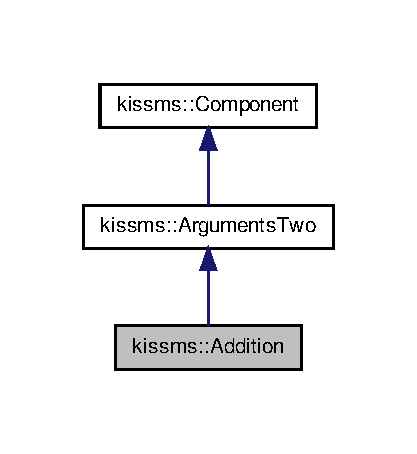
\includegraphics[width=200pt]{classkissms_1_1_addition__inherit__graph}
\end{center}
\end{figure}


Collaboration diagram for kissms\-:\-:Addition\-:
\nopagebreak
\begin{figure}[H]
\begin{center}
\leavevmode
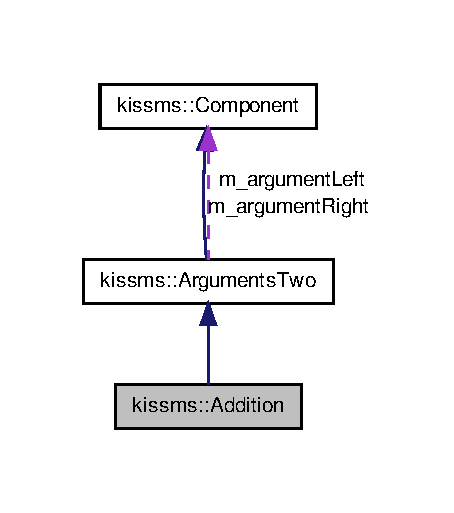
\includegraphics[width=218pt]{classkissms_1_1_addition__coll__graph}
\end{center}
\end{figure}
\subsection*{Additional Inherited Members}


\subsection{Detailed Description}


Definition at line 14 of file addition.\-h.



The documentation for this class was generated from the following file\-:\begin{DoxyCompactItemize}
\item 
/home/sieb/eclipse-\/workspace/eclipse-\/wrkspc\-\_\-\-F\-H/\-G\-D\-\_\-\-Phy\-Sim/src/kissms/component/scalar-\/two/\hyperlink{addition_8h}{addition.\-h}\end{DoxyCompactItemize}

\hypertarget{classkissms_1_1_arguments_one}{\section{kissms\-:\-:Arguments\-One Class Reference}
\label{classkissms_1_1_arguments_one}\index{kissms\-::\-Arguments\-One@{kissms\-::\-Arguments\-One}}
}


Representation of Components taking one argument.  




{\ttfamily \#include $<$arguments\-One.\-h$>$}



Inheritance diagram for kissms\-:\-:Arguments\-One\-:
\nopagebreak
\begin{figure}[H]
\begin{center}
\leavevmode
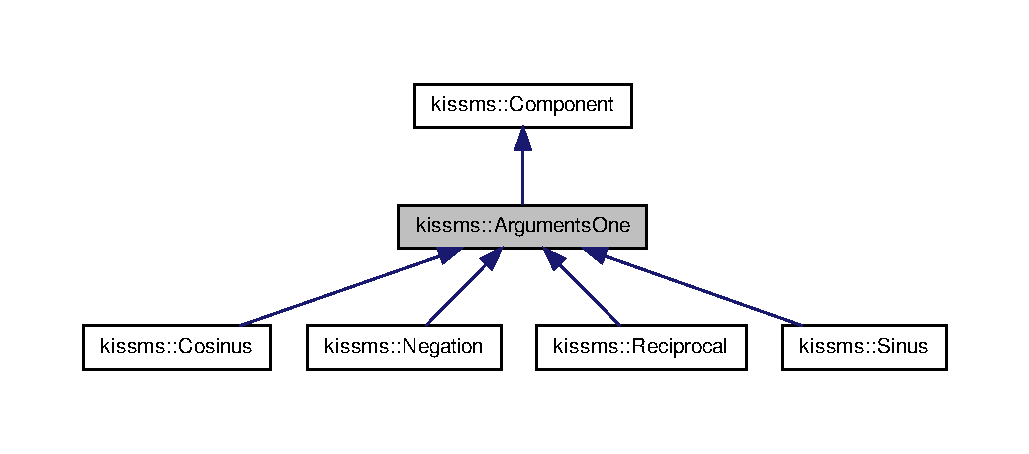
\includegraphics[width=350pt]{classkissms_1_1_arguments_one__inherit__graph}
\end{center}
\end{figure}


Collaboration diagram for kissms\-:\-:Arguments\-One\-:
\nopagebreak
\begin{figure}[H]
\begin{center}
\leavevmode
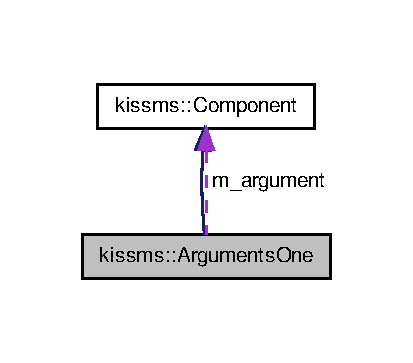
\includegraphics[width=198pt]{classkissms_1_1_arguments_one__coll__graph}
\end{center}
\end{figure}
\subsection*{Public Member Functions}
\begin{DoxyCompactItemize}
\item 
\hyperlink{classkissms_1_1_arguments_one_ad4bcc97fc91b51c8fbca79ce79e3403b}{Arguments\-One} ()
\item 
virtual \hyperlink{classkissms_1_1_arguments_one_aa340e54444664feca6977c521a2fb8c1}{$\sim$\-Arguments\-One} ()
\item 
void \hyperlink{classkissms_1_1_arguments_one_a96b3107c4779c1e5843a6fad91145f92}{set\-Argument} (\hyperlink{classkissms_1_1_component}{Component} $\ast$argument)
\begin{DoxyCompactList}\small\item\em Sets the \hyperlink{classkissms_1_1_component}{Component}'s argument. \end{DoxyCompactList}\end{DoxyCompactItemize}
\subsection*{Protected Attributes}
\begin{DoxyCompactItemize}
\item 
\hyperlink{classkissms_1_1_component}{Component} $\ast$ \hyperlink{classkissms_1_1_arguments_one_a13edd850fa593c54b343b4538b99a190}{m\-\_\-argument}
\begin{DoxyCompactList}\small\item\em The \hyperlink{classkissms_1_1_component}{Component}'s argument. \end{DoxyCompactList}\end{DoxyCompactItemize}


\subsection{Detailed Description}
Representation of Components taking one argument. 

Definition at line 19 of file arguments\-One.\-h.



\subsection{Constructor \& Destructor Documentation}
\hypertarget{classkissms_1_1_arguments_one_ad4bcc97fc91b51c8fbca79ce79e3403b}{\index{kissms\-::\-Arguments\-One@{kissms\-::\-Arguments\-One}!Arguments\-One@{Arguments\-One}}
\index{Arguments\-One@{Arguments\-One}!kissms::ArgumentsOne@{kissms\-::\-Arguments\-One}}
\subsubsection[{Arguments\-One}]{\setlength{\rightskip}{0pt plus 5cm}kissms\-::\-Arguments\-One\-::\-Arguments\-One (
\begin{DoxyParamCaption}
{}
\end{DoxyParamCaption}
)}}\label{classkissms_1_1_arguments_one_ad4bcc97fc91b51c8fbca79ce79e3403b}
\hypertarget{classkissms_1_1_arguments_one_aa340e54444664feca6977c521a2fb8c1}{\index{kissms\-::\-Arguments\-One@{kissms\-::\-Arguments\-One}!$\sim$\-Arguments\-One@{$\sim$\-Arguments\-One}}
\index{$\sim$\-Arguments\-One@{$\sim$\-Arguments\-One}!kissms::ArgumentsOne@{kissms\-::\-Arguments\-One}}
\subsubsection[{$\sim$\-Arguments\-One}]{\setlength{\rightskip}{0pt plus 5cm}virtual kissms\-::\-Arguments\-One\-::$\sim$\-Arguments\-One (
\begin{DoxyParamCaption}
{}
\end{DoxyParamCaption}
)\hspace{0.3cm}{\ttfamily [virtual]}}}\label{classkissms_1_1_arguments_one_aa340e54444664feca6977c521a2fb8c1}


\subsection{Member Function Documentation}
\hypertarget{classkissms_1_1_arguments_one_a96b3107c4779c1e5843a6fad91145f92}{\index{kissms\-::\-Arguments\-One@{kissms\-::\-Arguments\-One}!set\-Argument@{set\-Argument}}
\index{set\-Argument@{set\-Argument}!kissms::ArgumentsOne@{kissms\-::\-Arguments\-One}}
\subsubsection[{set\-Argument}]{\setlength{\rightskip}{0pt plus 5cm}void kissms\-::\-Arguments\-One\-::set\-Argument (
\begin{DoxyParamCaption}
\item[{{\bf Component} $\ast$}]{argument}
\end{DoxyParamCaption}
)}}\label{classkissms_1_1_arguments_one_a96b3107c4779c1e5843a6fad91145f92}


Sets the \hyperlink{classkissms_1_1_component}{Component}'s argument. 


\begin{DoxyParams}{Parameters}
{\em argument} & The \hyperlink{classkissms_1_1_component}{Component}'s new argument \\
\hline
\end{DoxyParams}


\subsection{Member Data Documentation}
\hypertarget{classkissms_1_1_arguments_one_a13edd850fa593c54b343b4538b99a190}{\index{kissms\-::\-Arguments\-One@{kissms\-::\-Arguments\-One}!m\-\_\-argument@{m\-\_\-argument}}
\index{m\-\_\-argument@{m\-\_\-argument}!kissms::ArgumentsOne@{kissms\-::\-Arguments\-One}}
\subsubsection[{m\-\_\-argument}]{\setlength{\rightskip}{0pt plus 5cm}{\bf Component}$\ast$ kissms\-::\-Arguments\-One\-::m\-\_\-argument\hspace{0.3cm}{\ttfamily [protected]}}}\label{classkissms_1_1_arguments_one_a13edd850fa593c54b343b4538b99a190}


The \hyperlink{classkissms_1_1_component}{Component}'s argument. 



Definition at line 35 of file arguments\-One.\-h.



The documentation for this class was generated from the following file\-:\begin{DoxyCompactItemize}
\item 
/home/sieb/eclipse-\/workspace/eclipse-\/wrkspc\-\_\-\-F\-H/\-G\-D\-\_\-\-Phy\-Sim/src/kissms/component/\hyperlink{arguments_one_8h}{arguments\-One.\-h}\end{DoxyCompactItemize}

\hypertarget{classkissms_1_1_arguments_two}{\section{kissms\-:\-:Arguments\-Two Class Reference}
\label{classkissms_1_1_arguments_two}\index{kissms\-::\-Arguments\-Two@{kissms\-::\-Arguments\-Two}}
}


Representation of Components taking two arguments.  




{\ttfamily \#include $<$arguments\-Two.\-h$>$}



Inheritance diagram for kissms\-:\-:Arguments\-Two\-:
\nopagebreak
\begin{figure}[H]
\begin{center}
\leavevmode
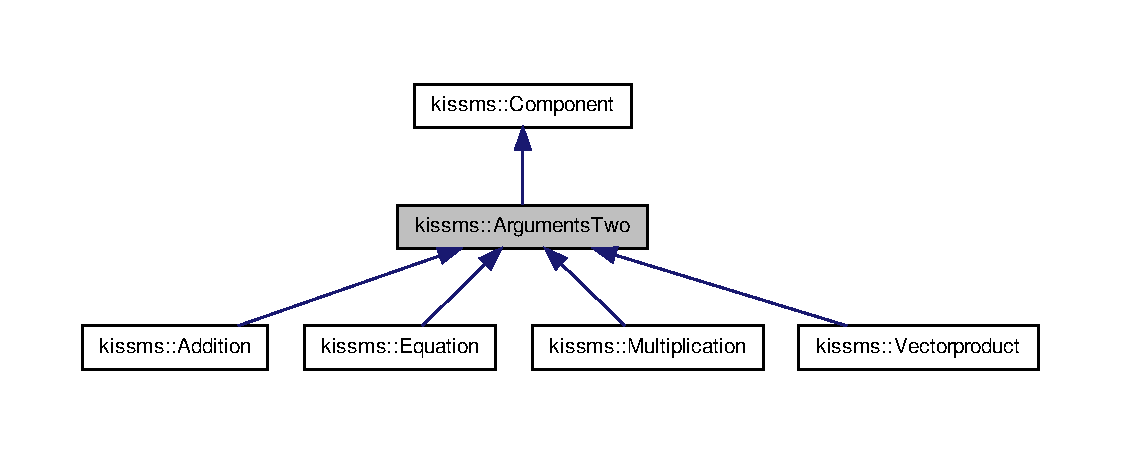
\includegraphics[width=350pt]{classkissms_1_1_arguments_two__inherit__graph}
\end{center}
\end{figure}


Collaboration diagram for kissms\-:\-:Arguments\-Two\-:
\nopagebreak
\begin{figure}[H]
\begin{center}
\leavevmode
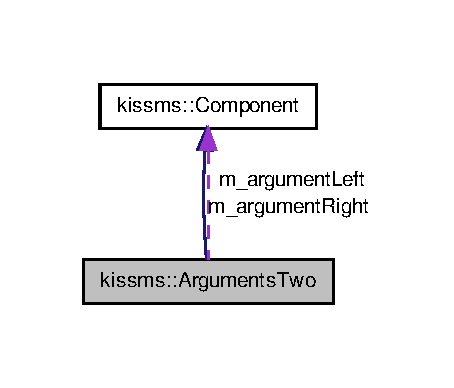
\includegraphics[width=218pt]{classkissms_1_1_arguments_two__coll__graph}
\end{center}
\end{figure}
\subsection*{Public Member Functions}
\begin{DoxyCompactItemize}
\item 
\hyperlink{classkissms_1_1_arguments_two_a8da02300ecb9eb1a6fc10dab83badd10}{Arguments\-Two} ()
\item 
virtual \hyperlink{classkissms_1_1_arguments_two_ab7ee206cc5dbd908336214030e7ff920}{$\sim$\-Arguments\-Two} ()
\item 
void \hyperlink{classkissms_1_1_arguments_two_a4abc6f6bca274e317a7d3b74c20e6e7c}{set\-Left} (\hyperlink{classkissms_1_1_component}{Component} $\ast$argument)
\begin{DoxyCompactList}\small\item\em Sets the \hyperlink{classkissms_1_1_component}{Component}'s left side. \end{DoxyCompactList}\item 
void \hyperlink{classkissms_1_1_arguments_two_a91446cdcdd8e907693c7e15f5f753e73}{set\-Right} (\hyperlink{classkissms_1_1_component}{Component} $\ast$argument)
\begin{DoxyCompactList}\small\item\em Sets the \hyperlink{classkissms_1_1_component}{Component}'s right side. \end{DoxyCompactList}\item 
void \hyperlink{classkissms_1_1_arguments_two_ac0e32475b1be1f5912da9af37346654e}{set\-Arguments} (\hyperlink{classkissms_1_1_component}{Component} $\ast$left, \hyperlink{classkissms_1_1_component}{Component} $\ast$right)
\begin{DoxyCompactList}\small\item\em Sets the \hyperlink{classkissms_1_1_component}{Component}'s arguments. \end{DoxyCompactList}\end{DoxyCompactItemize}
\subsection*{Protected Attributes}
\begin{DoxyCompactItemize}
\item 
\hyperlink{classkissms_1_1_component}{Component} $\ast$ \hyperlink{classkissms_1_1_arguments_two_a9c99ed4842c86cca7daec68e6184eefc}{m\-\_\-argument\-Left}
\begin{DoxyCompactList}\small\item\em The \hyperlink{classkissms_1_1_component}{Component}'s left side argument. \end{DoxyCompactList}\item 
\hyperlink{classkissms_1_1_component}{Component} $\ast$ \hyperlink{classkissms_1_1_arguments_two_a6c3c75623ef11c44443dc37b6574247e}{m\-\_\-argument\-Right}
\begin{DoxyCompactList}\small\item\em The \hyperlink{classkissms_1_1_component}{Component}'s right side argument. \end{DoxyCompactList}\end{DoxyCompactItemize}


\subsection{Detailed Description}
Representation of Components taking two arguments. 

Definition at line 19 of file arguments\-Two.\-h.



\subsection{Constructor \& Destructor Documentation}
\hypertarget{classkissms_1_1_arguments_two_a8da02300ecb9eb1a6fc10dab83badd10}{\index{kissms\-::\-Arguments\-Two@{kissms\-::\-Arguments\-Two}!Arguments\-Two@{Arguments\-Two}}
\index{Arguments\-Two@{Arguments\-Two}!kissms::ArgumentsTwo@{kissms\-::\-Arguments\-Two}}
\subsubsection[{Arguments\-Two}]{\setlength{\rightskip}{0pt plus 5cm}kissms\-::\-Arguments\-Two\-::\-Arguments\-Two (
\begin{DoxyParamCaption}
{}
\end{DoxyParamCaption}
)}}\label{classkissms_1_1_arguments_two_a8da02300ecb9eb1a6fc10dab83badd10}


Definition at line 12 of file arguments\-Two.\-cpp.

\hypertarget{classkissms_1_1_arguments_two_ab7ee206cc5dbd908336214030e7ff920}{\index{kissms\-::\-Arguments\-Two@{kissms\-::\-Arguments\-Two}!$\sim$\-Arguments\-Two@{$\sim$\-Arguments\-Two}}
\index{$\sim$\-Arguments\-Two@{$\sim$\-Arguments\-Two}!kissms::ArgumentsTwo@{kissms\-::\-Arguments\-Two}}
\subsubsection[{$\sim$\-Arguments\-Two}]{\setlength{\rightskip}{0pt plus 5cm}kissms\-::\-Arguments\-Two\-::$\sim$\-Arguments\-Two (
\begin{DoxyParamCaption}
{}
\end{DoxyParamCaption}
)\hspace{0.3cm}{\ttfamily [virtual]}}}\label{classkissms_1_1_arguments_two_ab7ee206cc5dbd908336214030e7ff920}


Definition at line 19 of file arguments\-Two.\-cpp.



\subsection{Member Function Documentation}
\hypertarget{classkissms_1_1_arguments_two_ac0e32475b1be1f5912da9af37346654e}{\index{kissms\-::\-Arguments\-Two@{kissms\-::\-Arguments\-Two}!set\-Arguments@{set\-Arguments}}
\index{set\-Arguments@{set\-Arguments}!kissms::ArgumentsTwo@{kissms\-::\-Arguments\-Two}}
\subsubsection[{set\-Arguments}]{\setlength{\rightskip}{0pt plus 5cm}void kissms\-::\-Arguments\-Two\-::set\-Arguments (
\begin{DoxyParamCaption}
\item[{{\bf Component} $\ast$}]{left, }
\item[{{\bf Component} $\ast$}]{right}
\end{DoxyParamCaption}
)}}\label{classkissms_1_1_arguments_two_ac0e32475b1be1f5912da9af37346654e}


Sets the \hyperlink{classkissms_1_1_component}{Component}'s arguments. 


\begin{DoxyParams}{Parameters}
{\em left} & New argument on the \hyperlink{classkissms_1_1_component}{Component}'s left side \\
\hline
{\em right} & New argument on the \hyperlink{classkissms_1_1_component}{Component}'s right side \\
\hline
\end{DoxyParams}
\hypertarget{classkissms_1_1_arguments_two_a4abc6f6bca274e317a7d3b74c20e6e7c}{\index{kissms\-::\-Arguments\-Two@{kissms\-::\-Arguments\-Two}!set\-Left@{set\-Left}}
\index{set\-Left@{set\-Left}!kissms::ArgumentsTwo@{kissms\-::\-Arguments\-Two}}
\subsubsection[{set\-Left}]{\setlength{\rightskip}{0pt plus 5cm}void kissms\-::\-Arguments\-Two\-::set\-Left (
\begin{DoxyParamCaption}
\item[{{\bf Component} $\ast$}]{argument}
\end{DoxyParamCaption}
)}}\label{classkissms_1_1_arguments_two_a4abc6f6bca274e317a7d3b74c20e6e7c}


Sets the \hyperlink{classkissms_1_1_component}{Component}'s left side. 


\begin{DoxyParams}{Parameters}
{\em argument} & New argument on the \hyperlink{classkissms_1_1_component}{Component}'s left side \\
\hline
\end{DoxyParams}
\hypertarget{classkissms_1_1_arguments_two_a91446cdcdd8e907693c7e15f5f753e73}{\index{kissms\-::\-Arguments\-Two@{kissms\-::\-Arguments\-Two}!set\-Right@{set\-Right}}
\index{set\-Right@{set\-Right}!kissms::ArgumentsTwo@{kissms\-::\-Arguments\-Two}}
\subsubsection[{set\-Right}]{\setlength{\rightskip}{0pt plus 5cm}void kissms\-::\-Arguments\-Two\-::set\-Right (
\begin{DoxyParamCaption}
\item[{{\bf Component} $\ast$}]{argument}
\end{DoxyParamCaption}
)}}\label{classkissms_1_1_arguments_two_a91446cdcdd8e907693c7e15f5f753e73}


Sets the \hyperlink{classkissms_1_1_component}{Component}'s right side. 


\begin{DoxyParams}{Parameters}
{\em argument} & New argument on the \hyperlink{classkissms_1_1_component}{Component}'s right side \\
\hline
\end{DoxyParams}


\subsection{Member Data Documentation}
\hypertarget{classkissms_1_1_arguments_two_a9c99ed4842c86cca7daec68e6184eefc}{\index{kissms\-::\-Arguments\-Two@{kissms\-::\-Arguments\-Two}!m\-\_\-argument\-Left@{m\-\_\-argument\-Left}}
\index{m\-\_\-argument\-Left@{m\-\_\-argument\-Left}!kissms::ArgumentsTwo@{kissms\-::\-Arguments\-Two}}
\subsubsection[{m\-\_\-argument\-Left}]{\setlength{\rightskip}{0pt plus 5cm}{\bf Component}$\ast$ kissms\-::\-Arguments\-Two\-::m\-\_\-argument\-Left\hspace{0.3cm}{\ttfamily [protected]}}}\label{classkissms_1_1_arguments_two_a9c99ed4842c86cca7daec68e6184eefc}


The \hyperlink{classkissms_1_1_component}{Component}'s left side argument. 



Definition at line 50 of file arguments\-Two.\-h.

\hypertarget{classkissms_1_1_arguments_two_a6c3c75623ef11c44443dc37b6574247e}{\index{kissms\-::\-Arguments\-Two@{kissms\-::\-Arguments\-Two}!m\-\_\-argument\-Right@{m\-\_\-argument\-Right}}
\index{m\-\_\-argument\-Right@{m\-\_\-argument\-Right}!kissms::ArgumentsTwo@{kissms\-::\-Arguments\-Two}}
\subsubsection[{m\-\_\-argument\-Right}]{\setlength{\rightskip}{0pt plus 5cm}{\bf Component}$\ast$ kissms\-::\-Arguments\-Two\-::m\-\_\-argument\-Right\hspace{0.3cm}{\ttfamily [protected]}}}\label{classkissms_1_1_arguments_two_a6c3c75623ef11c44443dc37b6574247e}


The \hyperlink{classkissms_1_1_component}{Component}'s right side argument. 



Definition at line 55 of file arguments\-Two.\-h.



The documentation for this class was generated from the following files\-:\begin{DoxyCompactItemize}
\item 
/home/sieb/eclipse-\/workspace/eclipse-\/wrkspc\-\_\-\-F\-H/\-G\-D\-\_\-\-Phy\-Sim/src/kissms/component/\hyperlink{arguments_two_8h}{arguments\-Two.\-h}\item 
/home/sieb/eclipse-\/workspace/eclipse-\/wrkspc\-\_\-\-F\-H/\-G\-D\-\_\-\-Phy\-Sim/src/kissms/component/\hyperlink{arguments_two_8cpp}{arguments\-Two.\-cpp}\end{DoxyCompactItemize}

\hypertarget{classkissms_1_1_component}{\section{kissms\-:\-:Component Class Reference}
\label{classkissms_1_1_component}\index{kissms\-::\-Component@{kissms\-::\-Component}}
}


Representation of a mathematical component in an \hyperlink{classkissms_1_1_equation}{Equation}.  




{\ttfamily \#include $<$component.\-h$>$}



Inheritance diagram for kissms\-:\-:Component\-:
\nopagebreak
\begin{figure}[H]
\begin{center}
\leavevmode
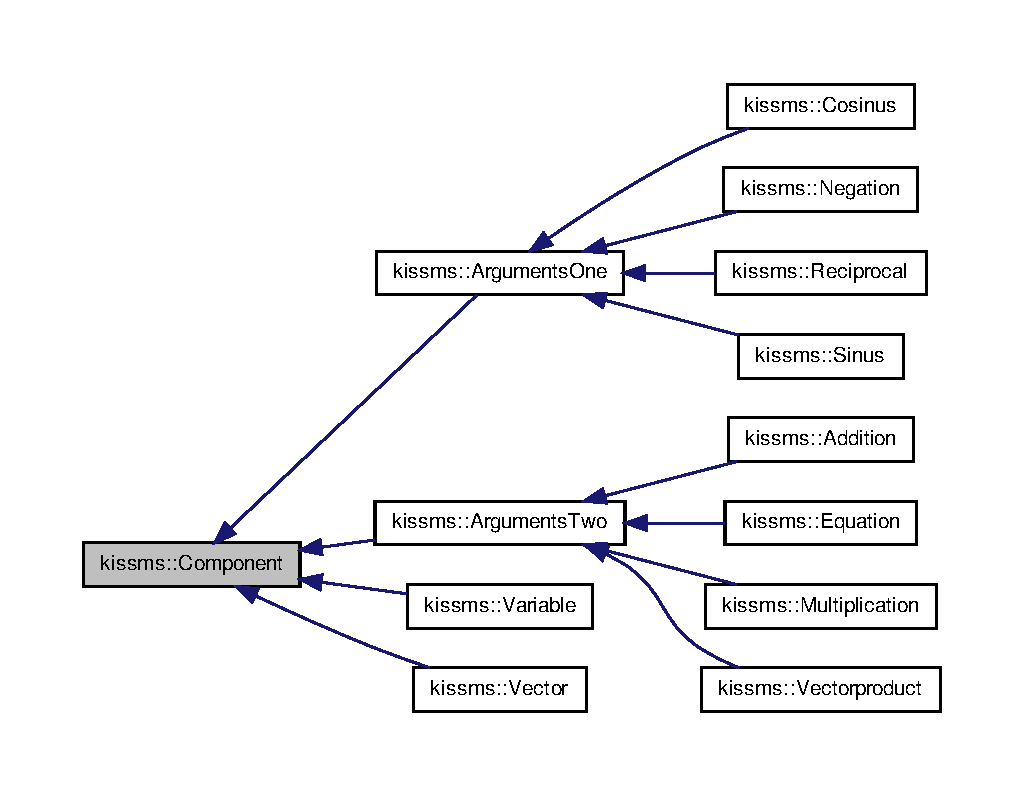
\includegraphics[width=350pt]{classkissms_1_1_component__inherit__graph}
\end{center}
\end{figure}
\subsection*{Public Member Functions}
\begin{DoxyCompactItemize}
\item 
\hyperlink{classkissms_1_1_component_ab5dbfef5bbb55dfbcc91de7cc70b78c7}{Component} ()
\item 
virtual \hyperlink{classkissms_1_1_component_a873c6f07a8fd5d4570dfd525fa703752}{$\sim$\-Component} ()
\item 
virtual bool \hyperlink{classkissms_1_1_component_a442885b45058f07566a0e52192f13cef}{is\-Calculable} ()=0
\begin{DoxyCompactList}\small\item\em Checks whether the \hyperlink{classkissms_1_1_component}{Component} is calculable. \end{DoxyCompactList}\item 
virtual bool \hyperlink{classkissms_1_1_component_aa919cd3999147b744975aea91c7d2928}{is\-Quantifiable} ()=0
\begin{DoxyCompactList}\small\item\em Checks whether the \hyperlink{classkissms_1_1_component}{Component} is representable by a numerical value. \end{DoxyCompactList}\item 
virtual \hyperlink{namespacekissms_a006cc132ffcae81e38527977e0846e0e}{Result\-Code} \hyperlink{classkissms_1_1_component_afed1b31c97ebe0113fc0890cbd50f005}{reform\-For} (\hyperlink{classkissms_1_1_variable}{Variable} $\ast$variable, \hyperlink{classkissms_1_1_component}{Component} $\ast$$\ast$new\-Side, \hyperlink{classkissms_1_1_component}{Component} $\ast$$\ast$other\-Side, \hyperlink{classkissms_1_1_component}{Component} $\ast$$\ast$placeholder)=0
\begin{DoxyCompactList}\small\item\em Returns Components for reformation. \end{DoxyCompactList}\item 
virtual \hyperlink{namespacekissms_a006cc132ffcae81e38527977e0846e0e}{Result\-Code} \hyperlink{classkissms_1_1_component_a256b837afb2726a85fe81a39599a35ff}{calculate} ()=0
\begin{DoxyCompactList}\small\item\em Calculates the \hyperlink{classkissms_1_1_component}{Component}'s numerical value. \end{DoxyCompactList}\end{DoxyCompactItemize}


\subsection{Detailed Description}
Representation of a mathematical component in an \hyperlink{classkissms_1_1_equation}{Equation}. 

Definition at line 19 of file component.\-h.



\subsection{Constructor \& Destructor Documentation}
\hypertarget{classkissms_1_1_component_ab5dbfef5bbb55dfbcc91de7cc70b78c7}{\index{kissms\-::\-Component@{kissms\-::\-Component}!Component@{Component}}
\index{Component@{Component}!kissms::Component@{kissms\-::\-Component}}
\subsubsection[{Component}]{\setlength{\rightskip}{0pt plus 5cm}kissms\-::\-Component\-::\-Component (
\begin{DoxyParamCaption}
{}
\end{DoxyParamCaption}
)}}\label{classkissms_1_1_component_ab5dbfef5bbb55dfbcc91de7cc70b78c7}


Definition at line 12 of file component.\-cpp.

\hypertarget{classkissms_1_1_component_a873c6f07a8fd5d4570dfd525fa703752}{\index{kissms\-::\-Component@{kissms\-::\-Component}!$\sim$\-Component@{$\sim$\-Component}}
\index{$\sim$\-Component@{$\sim$\-Component}!kissms::Component@{kissms\-::\-Component}}
\subsubsection[{$\sim$\-Component}]{\setlength{\rightskip}{0pt plus 5cm}kissms\-::\-Component\-::$\sim$\-Component (
\begin{DoxyParamCaption}
{}
\end{DoxyParamCaption}
)\hspace{0.3cm}{\ttfamily [virtual]}}}\label{classkissms_1_1_component_a873c6f07a8fd5d4570dfd525fa703752}


Definition at line 15 of file component.\-cpp.



\subsection{Member Function Documentation}
\hypertarget{classkissms_1_1_component_a256b837afb2726a85fe81a39599a35ff}{\index{kissms\-::\-Component@{kissms\-::\-Component}!calculate@{calculate}}
\index{calculate@{calculate}!kissms::Component@{kissms\-::\-Component}}
\subsubsection[{calculate}]{\setlength{\rightskip}{0pt plus 5cm}virtual {\bf Result\-Code} kissms\-::\-Component\-::calculate (
\begin{DoxyParamCaption}
{}
\end{DoxyParamCaption}
)\hspace{0.3cm}{\ttfamily [pure virtual]}}}\label{classkissms_1_1_component_a256b837afb2726a85fe81a39599a35ff}


Calculates the \hyperlink{classkissms_1_1_component}{Component}'s numerical value. 

\begin{DoxyReturn}{Returns}
Result\-Code
\end{DoxyReturn}
Calculates the \hyperlink{classkissms_1_1_component}{Component}'s numerical value as far as the \hyperlink{classkissms_1_1_component}{Component}'s childs allow this. 

Here is the caller graph for this function\-:
\nopagebreak
\begin{figure}[H]
\begin{center}
\leavevmode
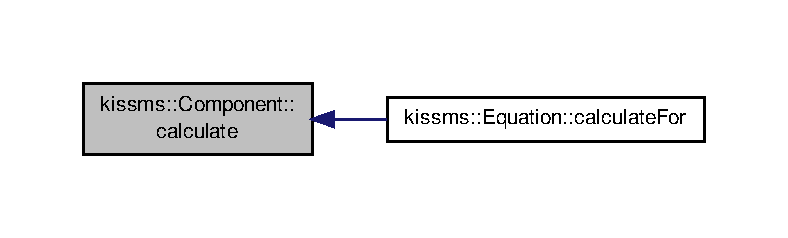
\includegraphics[width=350pt]{classkissms_1_1_component_a256b837afb2726a85fe81a39599a35ff_icgraph}
\end{center}
\end{figure}


\hypertarget{classkissms_1_1_component_a442885b45058f07566a0e52192f13cef}{\index{kissms\-::\-Component@{kissms\-::\-Component}!is\-Calculable@{is\-Calculable}}
\index{is\-Calculable@{is\-Calculable}!kissms::Component@{kissms\-::\-Component}}
\subsubsection[{is\-Calculable}]{\setlength{\rightskip}{0pt plus 5cm}virtual bool kissms\-::\-Component\-::is\-Calculable (
\begin{DoxyParamCaption}
{}
\end{DoxyParamCaption}
)\hspace{0.3cm}{\ttfamily [pure virtual]}}}\label{classkissms_1_1_component_a442885b45058f07566a0e52192f13cef}


Checks whether the \hyperlink{classkissms_1_1_component}{Component} is calculable. 


\begin{DoxyRetVals}{Return values}
{\em True} & The \hyperlink{classkissms_1_1_component}{Component} contains no unresolved Variables \\
\hline
{\em False} & The \hyperlink{classkissms_1_1_component}{Component} contains at least one unresolved \hyperlink{classkissms_1_1_variable}{Variable}\\
\hline
\end{DoxyRetVals}
Checks all child-\/\-Components for unresolved Variables. In case of finding at least one unresolved \hyperlink{classkissms_1_1_variable}{Variable} the \hyperlink{classkissms_1_1_component}{Component} is not calculable. Finding no unresolved Variables does not proove the \hyperlink{classkissms_1_1_component}{Component} as representable by a numerical value.

\begin{DoxySeeAlso}{See Also}
\hyperlink{classkissms_1_1_component_aa919cd3999147b744975aea91c7d2928}{is\-Quantifiable()} 
\end{DoxySeeAlso}


Implemented in \hyperlink{classkissms_1_1_variable_a9633a42cf7f3bb8542f705a881106393}{kissms\-::\-Variable}.



Here is the caller graph for this function\-:
\nopagebreak
\begin{figure}[H]
\begin{center}
\leavevmode
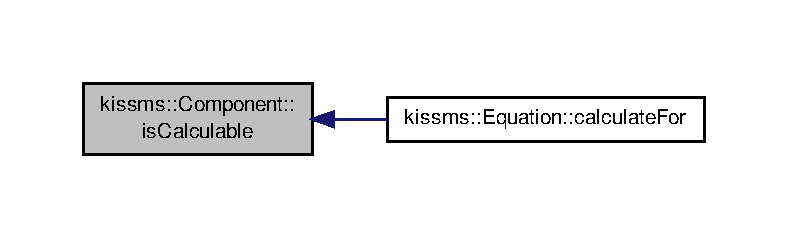
\includegraphics[width=350pt]{classkissms_1_1_component_a442885b45058f07566a0e52192f13cef_icgraph}
\end{center}
\end{figure}


\hypertarget{classkissms_1_1_component_aa919cd3999147b744975aea91c7d2928}{\index{kissms\-::\-Component@{kissms\-::\-Component}!is\-Quantifiable@{is\-Quantifiable}}
\index{is\-Quantifiable@{is\-Quantifiable}!kissms::Component@{kissms\-::\-Component}}
\subsubsection[{is\-Quantifiable}]{\setlength{\rightskip}{0pt plus 5cm}virtual bool kissms\-::\-Component\-::is\-Quantifiable (
\begin{DoxyParamCaption}
{}
\end{DoxyParamCaption}
)\hspace{0.3cm}{\ttfamily [pure virtual]}}}\label{classkissms_1_1_component_aa919cd3999147b744975aea91c7d2928}


Checks whether the \hyperlink{classkissms_1_1_component}{Component} is representable by a numerical value. 


\begin{DoxyRetVals}{Return values}
{\em True} & The \hyperlink{classkissms_1_1_component}{Component} is representable by a numerical value \\
\hline
{\em False} & The \hyperlink{classkissms_1_1_component}{Component} is not representable by a numerical value\\
\hline
\end{DoxyRetVals}
Checks all child-\/\-Components whether they are representable by numerical values.

\begin{DoxySeeAlso}{See Also}
\hyperlink{classkissms_1_1_component_a442885b45058f07566a0e52192f13cef}{is\-Calculable()} 
\end{DoxySeeAlso}


Implemented in \hyperlink{classkissms_1_1_variable_a7f12f0ed31f8ee613e50cf4c586c8fe3}{kissms\-::\-Variable}.

\hypertarget{classkissms_1_1_component_afed1b31c97ebe0113fc0890cbd50f005}{\index{kissms\-::\-Component@{kissms\-::\-Component}!reform\-For@{reform\-For}}
\index{reform\-For@{reform\-For}!kissms::Component@{kissms\-::\-Component}}
\subsubsection[{reform\-For}]{\setlength{\rightskip}{0pt plus 5cm}virtual {\bf Result\-Code} kissms\-::\-Component\-::reform\-For (
\begin{DoxyParamCaption}
\item[{{\bf Variable} $\ast$}]{variable, }
\item[{{\bf Component} $\ast$$\ast$}]{new\-Side, }
\item[{{\bf Component} $\ast$$\ast$}]{other\-Side, }
\item[{{\bf Component} $\ast$$\ast$}]{placeholder}
\end{DoxyParamCaption}
)\hspace{0.3cm}{\ttfamily [pure virtual]}}}\label{classkissms_1_1_component_afed1b31c97ebe0113fc0890cbd50f005}


Returns Components for reformation. 


\begin{DoxyParams}{Parameters}
{\em variable} & \hyperlink{classkissms_1_1_variable}{Variable} for which the \hyperlink{classkissms_1_1_component}{Component} shall reform itself \\
\hline
{\em new\-Side} & New \hyperlink{classkissms_1_1_component}{Component} replacing the \hyperlink{classkissms_1_1_component}{Component} on this side of the \hyperlink{classkissms_1_1_equation}{Equation} \\
\hline
{\em other\-Side} & \hyperlink{classkissms_1_1_component}{Component} for reformation of the \hyperlink{classkissms_1_1_equation}{Equation}'s other side \\
\hline
{\em placeholder} & Placeholder which shall be replaced by the \hyperlink{classkissms_1_1_equation}{Equation}'s old other side \\
\hline
\end{DoxyParams}
\begin{DoxyReturn}{Returns}
Result\-Code 
\end{DoxyReturn}


The documentation for this class was generated from the following files\-:\begin{DoxyCompactItemize}
\item 
/home/sieb/eclipse-\/workspace/eclipse-\/wrkspc\-\_\-\-F\-H/\-G\-D\-\_\-\-Phy\-Sim/src/kissms/component/\hyperlink{component_8h}{component.\-h}\item 
/home/sieb/eclipse-\/workspace/eclipse-\/wrkspc\-\_\-\-F\-H/\-G\-D\-\_\-\-Phy\-Sim/src/kissms/component/\hyperlink{component_8cpp}{component.\-cpp}\end{DoxyCompactItemize}

\hypertarget{classkissms_1_1_constant}{\section{kissms\-:\-:Constant Class Reference}
\label{classkissms_1_1_constant}\index{kissms\-::\-Constant@{kissms\-::\-Constant}}
}


{\ttfamily \#include $<$constant.\-h$>$}



\subsection{Detailed Description}


Definition at line 14 of file constant.\-h.



The documentation for this class was generated from the following file\-:\begin{DoxyCompactItemize}
\item 
/home/sieb/eclipse-\/workspace/eclipse-\/wrkspc\-\_\-\-F\-H/\-G\-D\-\_\-\-Phy\-Sim/src/kissms/component/scalar-\/leaf/\hyperlink{constant_8h}{constant.\-h}\end{DoxyCompactItemize}

\hypertarget{classkissms_1_1_cosinus}{\section{kissms\-:\-:Cosinus Class Reference}
\label{classkissms_1_1_cosinus}\index{kissms\-::\-Cosinus@{kissms\-::\-Cosinus}}
}


{\ttfamily \#include $<$cosinus.\-h$>$}



Inheritance diagram for kissms\-:\-:Cosinus\-:
\nopagebreak
\begin{figure}[H]
\begin{center}
\leavevmode
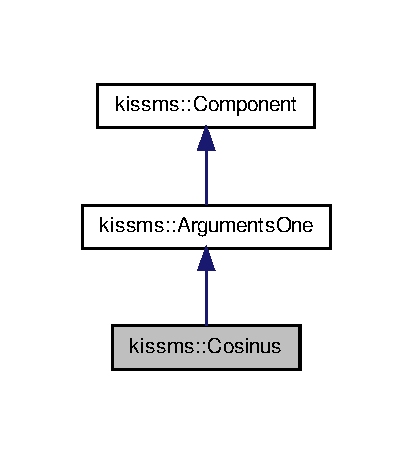
\includegraphics[width=198pt]{classkissms_1_1_cosinus__inherit__graph}
\end{center}
\end{figure}


Collaboration diagram for kissms\-:\-:Cosinus\-:
\nopagebreak
\begin{figure}[H]
\begin{center}
\leavevmode
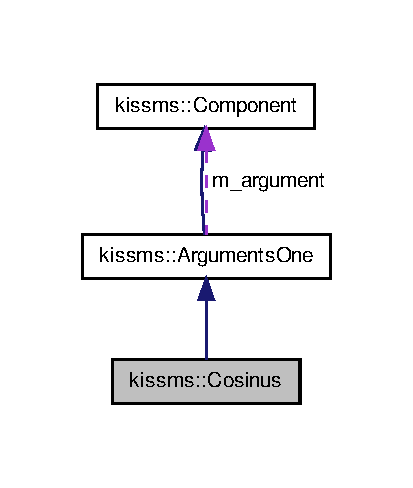
\includegraphics[width=198pt]{classkissms_1_1_cosinus__coll__graph}
\end{center}
\end{figure}
\subsection*{Additional Inherited Members}


\subsection{Detailed Description}


Definition at line 14 of file cosinus.\-h.



The documentation for this class was generated from the following file\-:\begin{DoxyCompactItemize}
\item 
/home/sieb/eclipse-\/workspace/eclipse-\/wrkspc\-\_\-\-F\-H/\-G\-D\-\_\-\-Phy\-Sim/src/kissms/component/scalar-\/one/\hyperlink{cosinus_8h}{cosinus.\-h}\end{DoxyCompactItemize}

\hypertarget{classkissms_1_1_equation}{\section{kissms\-:\-:Equation Class Reference}
\label{classkissms_1_1_equation}\index{kissms\-::\-Equation@{kissms\-::\-Equation}}
}


\hyperlink{classkissms_1_1_component}{Component} representing a whole mathematical equation.  




{\ttfamily \#include $<$equation.\-h$>$}



Inheritance diagram for kissms\-:\-:Equation\-:
\nopagebreak
\begin{figure}[H]
\begin{center}
\leavevmode
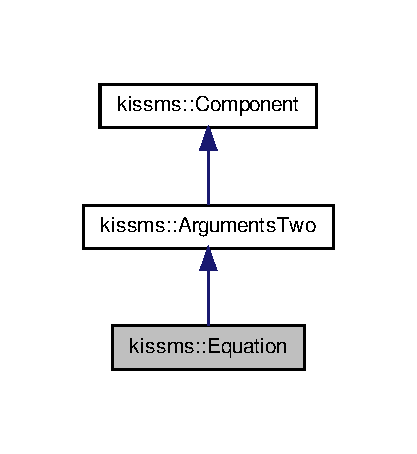
\includegraphics[width=200pt]{classkissms_1_1_equation__inherit__graph}
\end{center}
\end{figure}


Collaboration diagram for kissms\-:\-:Equation\-:
\nopagebreak
\begin{figure}[H]
\begin{center}
\leavevmode
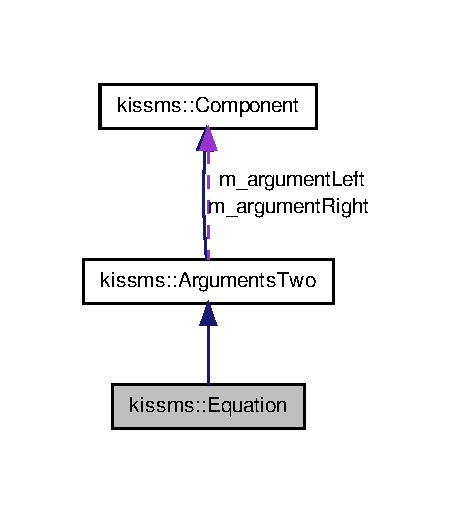
\includegraphics[width=218pt]{classkissms_1_1_equation__coll__graph}
\end{center}
\end{figure}
\subsection*{Public Member Functions}
\begin{DoxyCompactItemize}
\item 
\hyperlink{classkissms_1_1_equation_a222c08c6b55679b4808f7b807ac94184}{Equation} ()
\item 
virtual \hyperlink{classkissms_1_1_equation_ac0c9135b48a8f09ff4ffc0b60cad9c0a}{$\sim$\-Equation} ()
\item 
\hyperlink{namespacekissms_a006cc132ffcae81e38527977e0846e0e}{Result\-Code} \hyperlink{classkissms_1_1_equation_ad2a8ce5aff621d4e19b5042fcedf04de}{solve\-For} (\hyperlink{classkissms_1_1_variable}{Variable} $\ast$variable)
\begin{DoxyCompactList}\small\item\em Solves the \hyperlink{classkissms_1_1_equation}{Equation}. \end{DoxyCompactList}\item 
\hyperlink{namespacekissms_a006cc132ffcae81e38527977e0846e0e}{Result\-Code} \hyperlink{classkissms_1_1_equation_a72474be0471c6190f8cc3d6f5016b115}{calculate\-For} (\hyperlink{classkissms_1_1_variable}{Variable} $\ast$variable)
\begin{DoxyCompactList}\small\item\em Solves and calculates the \hyperlink{classkissms_1_1_equation}{Equation}. \end{DoxyCompactList}\item 
bool \hyperlink{classkissms_1_1_equation_a6f6ded9239ff0a8ec9792e0450d205f1}{contains} (\hyperlink{classkissms_1_1_variable}{Variable} $\ast$variable)
\begin{DoxyCompactList}\small\item\em Checks whether the \hyperlink{classkissms_1_1_equation}{Equation} contains a given \hyperlink{classkissms_1_1_variable}{Variable}. \end{DoxyCompactList}\end{DoxyCompactItemize}
\subsection*{Additional Inherited Members}


\subsection{Detailed Description}
\hyperlink{classkissms_1_1_component}{Component} representing a whole mathematical equation. 

Definition at line 17 of file equation.\-h.



\subsection{Constructor \& Destructor Documentation}
\hypertarget{classkissms_1_1_equation_a222c08c6b55679b4808f7b807ac94184}{\index{kissms\-::\-Equation@{kissms\-::\-Equation}!Equation@{Equation}}
\index{Equation@{Equation}!kissms::Equation@{kissms\-::\-Equation}}
\subsubsection[{Equation}]{\setlength{\rightskip}{0pt plus 5cm}kissms\-::\-Equation\-::\-Equation (
\begin{DoxyParamCaption}
{}
\end{DoxyParamCaption}
)}}\label{classkissms_1_1_equation_a222c08c6b55679b4808f7b807ac94184}


Definition at line 12 of file equation.\-cpp.

\hypertarget{classkissms_1_1_equation_ac0c9135b48a8f09ff4ffc0b60cad9c0a}{\index{kissms\-::\-Equation@{kissms\-::\-Equation}!$\sim$\-Equation@{$\sim$\-Equation}}
\index{$\sim$\-Equation@{$\sim$\-Equation}!kissms::Equation@{kissms\-::\-Equation}}
\subsubsection[{$\sim$\-Equation}]{\setlength{\rightskip}{0pt plus 5cm}kissms\-::\-Equation\-::$\sim$\-Equation (
\begin{DoxyParamCaption}
{}
\end{DoxyParamCaption}
)\hspace{0.3cm}{\ttfamily [virtual]}}}\label{classkissms_1_1_equation_ac0c9135b48a8f09ff4ffc0b60cad9c0a}


Definition at line 15 of file equation.\-cpp.



\subsection{Member Function Documentation}
\hypertarget{classkissms_1_1_equation_a72474be0471c6190f8cc3d6f5016b115}{\index{kissms\-::\-Equation@{kissms\-::\-Equation}!calculate\-For@{calculate\-For}}
\index{calculate\-For@{calculate\-For}!kissms::Equation@{kissms\-::\-Equation}}
\subsubsection[{calculate\-For}]{\setlength{\rightskip}{0pt plus 5cm}{\bf Result\-Code} kissms\-::\-Equation\-::calculate\-For (
\begin{DoxyParamCaption}
\item[{{\bf Variable} $\ast$}]{variable}
\end{DoxyParamCaption}
)}}\label{classkissms_1_1_equation_a72474be0471c6190f8cc3d6f5016b115}


Solves and calculates the \hyperlink{classkissms_1_1_equation}{Equation}. 


\begin{DoxyParams}{Parameters}
{\em variable} & \hyperlink{classkissms_1_1_variable}{Variable} for which the \hyperlink{classkissms_1_1_equation}{Equation} shall be solved \\
\hline
\end{DoxyParams}
\begin{DoxyReturn}{Returns}
Result\-Code
\end{DoxyReturn}
The \hyperlink{classkissms_1_1_equation}{Equation} is solved using \hyperlink{classkissms_1_1_equation_ad2a8ce5aff621d4e19b5042fcedf04de}{solve\-For()} and afterwards the \hyperlink{classkissms_1_1_variable}{Variable}'s value will be calculated, as far as the \hyperlink{classkissms_1_1_equation}{Equation}'s other side allows it.

\begin{DoxySeeAlso}{See Also}
\hyperlink{classkissms_1_1_equation_ad2a8ce5aff621d4e19b5042fcedf04de}{solve\-For( Variable $\ast$variable )} 
\end{DoxySeeAlso}


Definition at line 34 of file equation.\-cpp.



Here is the call graph for this function\-:
\nopagebreak
\begin{figure}[H]
\begin{center}
\leavevmode
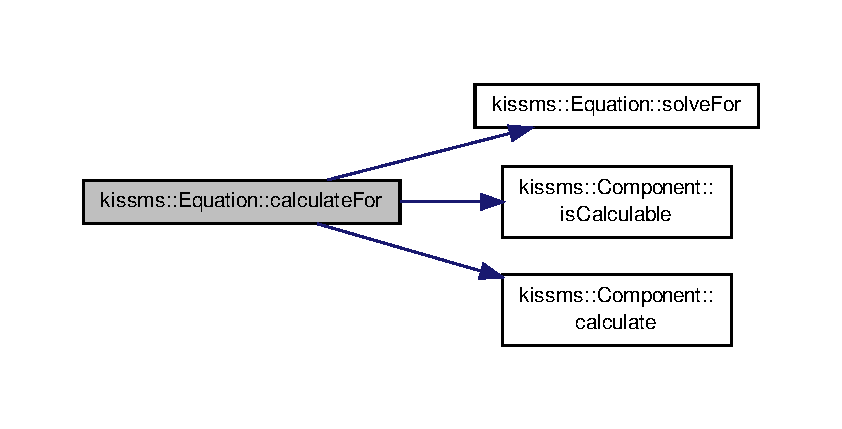
\includegraphics[width=350pt]{classkissms_1_1_equation_a72474be0471c6190f8cc3d6f5016b115_cgraph}
\end{center}
\end{figure}


\hypertarget{classkissms_1_1_equation_a6f6ded9239ff0a8ec9792e0450d205f1}{\index{kissms\-::\-Equation@{kissms\-::\-Equation}!contains@{contains}}
\index{contains@{contains}!kissms::Equation@{kissms\-::\-Equation}}
\subsubsection[{contains}]{\setlength{\rightskip}{0pt plus 5cm}bool kissms\-::\-Equation\-::contains (
\begin{DoxyParamCaption}
\item[{{\bf Variable} $\ast$}]{variable}
\end{DoxyParamCaption}
)}}\label{classkissms_1_1_equation_a6f6ded9239ff0a8ec9792e0450d205f1}


Checks whether the \hyperlink{classkissms_1_1_equation}{Equation} contains a given \hyperlink{classkissms_1_1_variable}{Variable}. 


\begin{DoxyParams}{Parameters}
{\em variable} & \hyperlink{classkissms_1_1_variable}{Variable} to check for \\
\hline
\end{DoxyParams}


Definition at line 62 of file equation.\-cpp.

\hypertarget{classkissms_1_1_equation_ad2a8ce5aff621d4e19b5042fcedf04de}{\index{kissms\-::\-Equation@{kissms\-::\-Equation}!solve\-For@{solve\-For}}
\index{solve\-For@{solve\-For}!kissms::Equation@{kissms\-::\-Equation}}
\subsubsection[{solve\-For}]{\setlength{\rightskip}{0pt plus 5cm}{\bf Result\-Code} kissms\-::\-Equation\-::solve\-For (
\begin{DoxyParamCaption}
\item[{{\bf Variable} $\ast$}]{variable}
\end{DoxyParamCaption}
)}}\label{classkissms_1_1_equation_ad2a8ce5aff621d4e19b5042fcedf04de}


Solves the \hyperlink{classkissms_1_1_equation}{Equation}. 


\begin{DoxyParams}{Parameters}
{\em variable} & \hyperlink{classkissms_1_1_variable}{Variable} for which the \hyperlink{classkissms_1_1_equation}{Equation} shall be solved \\
\hline
\end{DoxyParams}
\begin{DoxyReturn}{Returns}
Result\-Code
\end{DoxyReturn}
The \hyperlink{classkissms_1_1_equation}{Equation} is reformed so that the given \hyperlink{classkissms_1_1_variable}{Variable} is explicitely represented by the \hyperlink{classkissms_1_1_equation}{Equation}'s other side. The \hyperlink{classkissms_1_1_variable}{Variable}'s actual value won't be calculated.

\begin{DoxySeeAlso}{See Also}
\hyperlink{classkissms_1_1_equation_a72474be0471c6190f8cc3d6f5016b115}{calculate\-For()} 
\end{DoxySeeAlso}


Definition at line 18 of file equation.\-cpp.



Here is the caller graph for this function\-:
\nopagebreak
\begin{figure}[H]
\begin{center}
\leavevmode
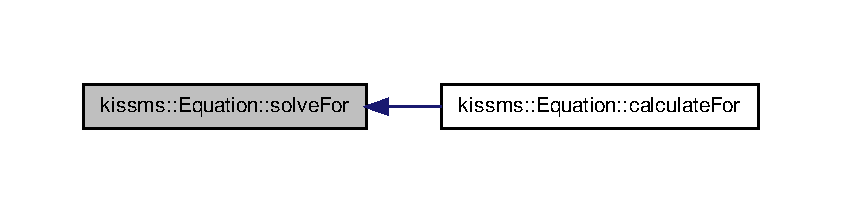
\includegraphics[width=350pt]{classkissms_1_1_equation_ad2a8ce5aff621d4e19b5042fcedf04de_icgraph}
\end{center}
\end{figure}




The documentation for this class was generated from the following files\-:\begin{DoxyCompactItemize}
\item 
/home/sieb/eclipse-\/workspace/eclipse-\/wrkspc\-\_\-\-F\-H/\-G\-D\-\_\-\-Phy\-Sim/src/kissms/\hyperlink{equation_8h}{equation.\-h}\item 
/home/sieb/eclipse-\/workspace/eclipse-\/wrkspc\-\_\-\-F\-H/\-G\-D\-\_\-\-Phy\-Sim/src/kissms/\hyperlink{equation_8cpp}{equation.\-cpp}\end{DoxyCompactItemize}

\hypertarget{classkissms_1_1_multiplication}{\section{kissms\-:\-:Multiplication Class Reference}
\label{classkissms_1_1_multiplication}\index{kissms\-::\-Multiplication@{kissms\-::\-Multiplication}}
}


{\ttfamily \#include $<$multiplication.\-h$>$}



Inheritance diagram for kissms\-:\-:Multiplication\-:
\nopagebreak
\begin{figure}[H]
\begin{center}
\leavevmode
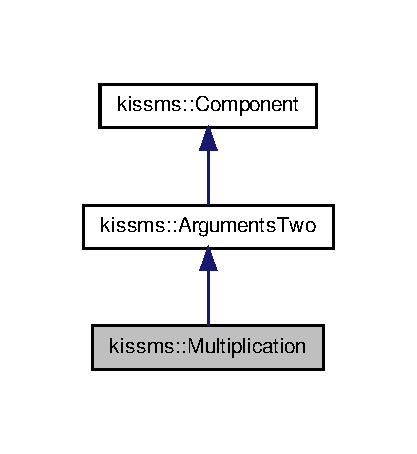
\includegraphics[width=200pt]{classkissms_1_1_multiplication__inherit__graph}
\end{center}
\end{figure}


Collaboration diagram for kissms\-:\-:Multiplication\-:
\nopagebreak
\begin{figure}[H]
\begin{center}
\leavevmode
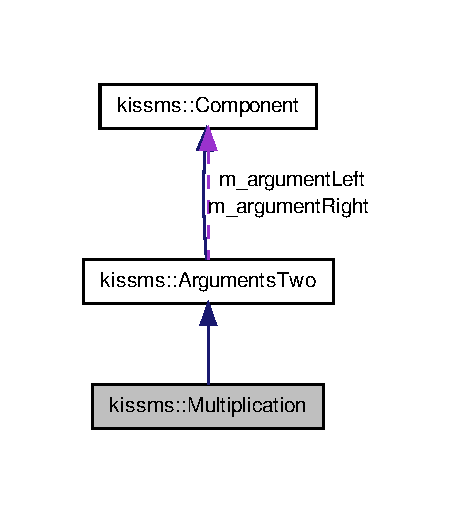
\includegraphics[width=218pt]{classkissms_1_1_multiplication__coll__graph}
\end{center}
\end{figure}
\subsection*{Additional Inherited Members}


\subsection{Detailed Description}


Definition at line 14 of file multiplication.\-h.



The documentation for this class was generated from the following file\-:\begin{DoxyCompactItemize}
\item 
/home/sieb/eclipse-\/workspace/eclipse-\/wrkspc\-\_\-\-F\-H/\-G\-D\-\_\-\-Phy\-Sim/src/kissms/component/scalar-\/two/\hyperlink{multiplication_8h}{multiplication.\-h}\end{DoxyCompactItemize}

\hypertarget{classkissms_1_1_negation}{\section{kissms\-:\-:Negation Class Reference}
\label{classkissms_1_1_negation}\index{kissms\-::\-Negation@{kissms\-::\-Negation}}
}


{\ttfamily \#include $<$negation.\-h$>$}



Inheritance diagram for kissms\-:\-:Negation\-:
\nopagebreak
\begin{figure}[H]
\begin{center}
\leavevmode
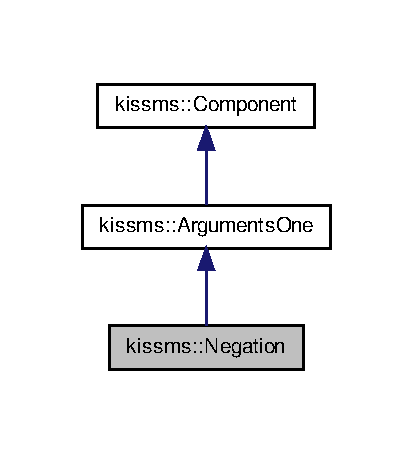
\includegraphics[width=198pt]{classkissms_1_1_negation__inherit__graph}
\end{center}
\end{figure}


Collaboration diagram for kissms\-:\-:Negation\-:
\nopagebreak
\begin{figure}[H]
\begin{center}
\leavevmode
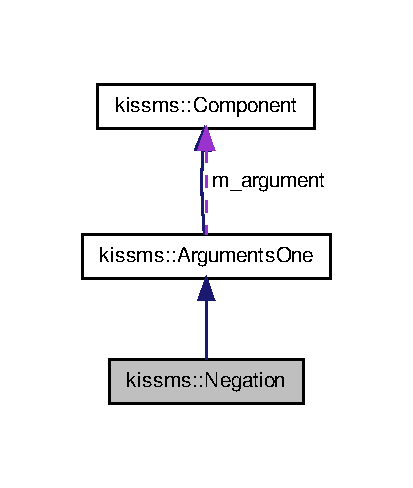
\includegraphics[width=198pt]{classkissms_1_1_negation__coll__graph}
\end{center}
\end{figure}
\subsection*{Additional Inherited Members}


\subsection{Detailed Description}


Definition at line 14 of file negation.\-h.



The documentation for this class was generated from the following file\-:\begin{DoxyCompactItemize}
\item 
/home/sieb/eclipse-\/workspace/eclipse-\/wrkspc\-\_\-\-F\-H/\-G\-D\-\_\-\-Phy\-Sim/src/kissms/component/scalar-\/one/\hyperlink{negation_8h}{negation.\-h}\end{DoxyCompactItemize}

\hypertarget{classkissms_1_1_reciprocal}{\section{kissms\-:\-:Reciprocal Class Reference}
\label{classkissms_1_1_reciprocal}\index{kissms\-::\-Reciprocal@{kissms\-::\-Reciprocal}}
}


{\ttfamily \#include $<$reciprocal.\-h$>$}



Inheritance diagram for kissms\-:\-:Reciprocal\-:
\nopagebreak
\begin{figure}[H]
\begin{center}
\leavevmode
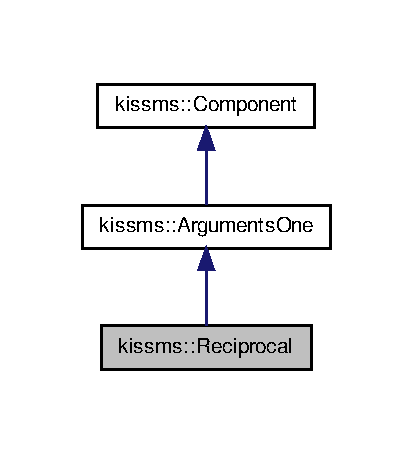
\includegraphics[width=198pt]{classkissms_1_1_reciprocal__inherit__graph}
\end{center}
\end{figure}


Collaboration diagram for kissms\-:\-:Reciprocal\-:
\nopagebreak
\begin{figure}[H]
\begin{center}
\leavevmode
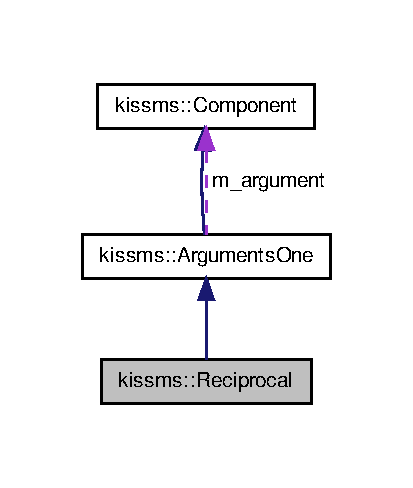
\includegraphics[width=198pt]{classkissms_1_1_reciprocal__coll__graph}
\end{center}
\end{figure}
\subsection*{Additional Inherited Members}


\subsection{Detailed Description}


Definition at line 14 of file reciprocal.\-h.



The documentation for this class was generated from the following file\-:\begin{DoxyCompactItemize}
\item 
/home/sieb/eclipse-\/workspace/eclipse-\/wrkspc\-\_\-\-F\-H/\-G\-D\-\_\-\-Phy\-Sim/src/kissms/component/scalar-\/one/\hyperlink{reciprocal_8h}{reciprocal.\-h}\end{DoxyCompactItemize}

\hypertarget{classkissms_1_1_sinus}{\section{kissms\-:\-:Sinus Class Reference}
\label{classkissms_1_1_sinus}\index{kissms\-::\-Sinus@{kissms\-::\-Sinus}}
}


{\ttfamily \#include $<$sinus.\-h$>$}



Inheritance diagram for kissms\-:\-:Sinus\-:
\nopagebreak
\begin{figure}[H]
\begin{center}
\leavevmode
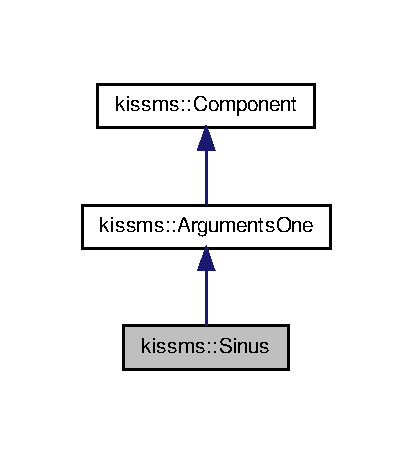
\includegraphics[width=198pt]{classkissms_1_1_sinus__inherit__graph}
\end{center}
\end{figure}


Collaboration diagram for kissms\-:\-:Sinus\-:
\nopagebreak
\begin{figure}[H]
\begin{center}
\leavevmode
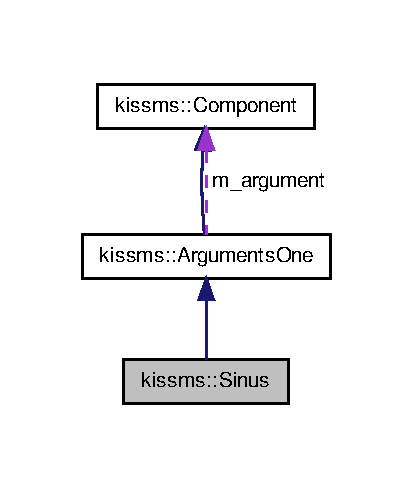
\includegraphics[width=198pt]{classkissms_1_1_sinus__coll__graph}
\end{center}
\end{figure}
\subsection*{Additional Inherited Members}


\subsection{Detailed Description}


Definition at line 14 of file sinus.\-h.



The documentation for this class was generated from the following file\-:\begin{DoxyCompactItemize}
\item 
/home/sieb/eclipse-\/workspace/eclipse-\/wrkspc\-\_\-\-F\-H/\-G\-D\-\_\-\-Phy\-Sim/src/kissms/component/scalar-\/one/\hyperlink{sinus_8h}{sinus.\-h}\end{DoxyCompactItemize}

\hypertarget{classkissms_1_1_variable}{\section{kissms\-:\-:Variable Class Reference}
\label{classkissms_1_1_variable}\index{kissms\-::\-Variable@{kissms\-::\-Variable}}
}


\hyperlink{classkissms_1_1_component}{Component} representing a single variable value.  




{\ttfamily \#include $<$variable.\-h$>$}



Inheritance diagram for kissms\-:\-:Variable\-:
\nopagebreak
\begin{figure}[H]
\begin{center}
\leavevmode
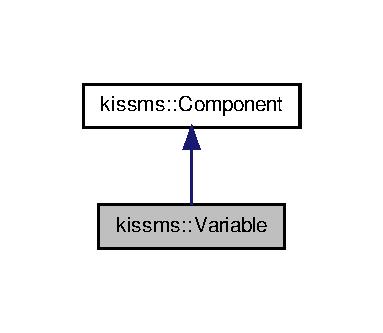
\includegraphics[width=184pt]{classkissms_1_1_variable__inherit__graph}
\end{center}
\end{figure}


Collaboration diagram for kissms\-:\-:Variable\-:
\nopagebreak
\begin{figure}[H]
\begin{center}
\leavevmode
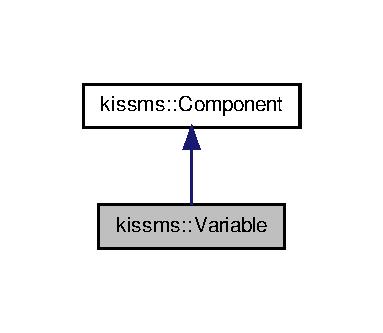
\includegraphics[width=184pt]{classkissms_1_1_variable__coll__graph}
\end{center}
\end{figure}
\subsection*{Public Member Functions}
\begin{DoxyCompactItemize}
\item 
\hyperlink{classkissms_1_1_variable_abb117c861a38d6ad571a4d0c9572f959}{Variable} ()
\item 
virtual \hyperlink{classkissms_1_1_variable_a53b44b419d55654020b6d0d655bc2f38}{$\sim$\-Variable} ()
\item 
void \hyperlink{classkissms_1_1_variable_a963a7b41e6156d3144ddcfba37201872}{set\-Variable} (char $\ast$name)
\begin{DoxyCompactList}\small\item\em Set the \hyperlink{classkissms_1_1_variable}{Variable}'s name. \end{DoxyCompactList}\item 
virtual bool \hyperlink{classkissms_1_1_variable_a9633a42cf7f3bb8542f705a881106393}{is\-Calculable} ()
\begin{DoxyCompactList}\small\item\em Checks whether the \hyperlink{classkissms_1_1_component}{Component} is calculable. \end{DoxyCompactList}\item 
virtual bool \hyperlink{classkissms_1_1_variable_a7f12f0ed31f8ee613e50cf4c586c8fe3}{is\-Quantifiable} ()
\begin{DoxyCompactList}\small\item\em Checks whether the \hyperlink{classkissms_1_1_component}{Component} is representable by a numerical value. \end{DoxyCompactList}\end{DoxyCompactItemize}


\subsection{Detailed Description}
\hyperlink{classkissms_1_1_component}{Component} representing a single variable value. 

Definition at line 17 of file variable.\-h.



\subsection{Constructor \& Destructor Documentation}
\hypertarget{classkissms_1_1_variable_abb117c861a38d6ad571a4d0c9572f959}{\index{kissms\-::\-Variable@{kissms\-::\-Variable}!Variable@{Variable}}
\index{Variable@{Variable}!kissms::Variable@{kissms\-::\-Variable}}
\subsubsection[{Variable}]{\setlength{\rightskip}{0pt plus 5cm}kissms\-::\-Variable\-::\-Variable (
\begin{DoxyParamCaption}
{}
\end{DoxyParamCaption}
)}}\label{classkissms_1_1_variable_abb117c861a38d6ad571a4d0c9572f959}


Definition at line 12 of file variable.\-cpp.

\hypertarget{classkissms_1_1_variable_a53b44b419d55654020b6d0d655bc2f38}{\index{kissms\-::\-Variable@{kissms\-::\-Variable}!$\sim$\-Variable@{$\sim$\-Variable}}
\index{$\sim$\-Variable@{$\sim$\-Variable}!kissms::Variable@{kissms\-::\-Variable}}
\subsubsection[{$\sim$\-Variable}]{\setlength{\rightskip}{0pt plus 5cm}kissms\-::\-Variable\-::$\sim$\-Variable (
\begin{DoxyParamCaption}
{}
\end{DoxyParamCaption}
)\hspace{0.3cm}{\ttfamily [virtual]}}}\label{classkissms_1_1_variable_a53b44b419d55654020b6d0d655bc2f38}


Definition at line 15 of file variable.\-cpp.



\subsection{Member Function Documentation}
\hypertarget{classkissms_1_1_variable_a9633a42cf7f3bb8542f705a881106393}{\index{kissms\-::\-Variable@{kissms\-::\-Variable}!is\-Calculable@{is\-Calculable}}
\index{is\-Calculable@{is\-Calculable}!kissms::Variable@{kissms\-::\-Variable}}
\subsubsection[{is\-Calculable}]{\setlength{\rightskip}{0pt plus 5cm}bool kissms\-::\-Variable\-::is\-Calculable (
\begin{DoxyParamCaption}
{}
\end{DoxyParamCaption}
)\hspace{0.3cm}{\ttfamily [virtual]}}}\label{classkissms_1_1_variable_a9633a42cf7f3bb8542f705a881106393}


Checks whether the \hyperlink{classkissms_1_1_component}{Component} is calculable. 


\begin{DoxyRetVals}{Return values}
{\em True} & The \hyperlink{classkissms_1_1_component}{Component} contains no unresolved Variables \\
\hline
{\em False} & The \hyperlink{classkissms_1_1_component}{Component} contains at least one unresolved \hyperlink{classkissms_1_1_variable}{Variable}\\
\hline
\end{DoxyRetVals}
Checks all child-\/\-Components for unresolved Variables. In case of finding at least one unresolved \hyperlink{classkissms_1_1_variable}{Variable} the \hyperlink{classkissms_1_1_component}{Component} is not calculable. Finding no unresolved Variables does not proove the \hyperlink{classkissms_1_1_component}{Component} as representable by a numerical value.

\begin{DoxySeeAlso}{See Also}
\hyperlink{classkissms_1_1_variable_a7f12f0ed31f8ee613e50cf4c586c8fe3}{is\-Quantifiable()} 
\end{DoxySeeAlso}


Implements \hyperlink{classkissms_1_1_component_a442885b45058f07566a0e52192f13cef}{kissms\-::\-Component}.



Definition at line 21 of file variable.\-cpp.

\hypertarget{classkissms_1_1_variable_a7f12f0ed31f8ee613e50cf4c586c8fe3}{\index{kissms\-::\-Variable@{kissms\-::\-Variable}!is\-Quantifiable@{is\-Quantifiable}}
\index{is\-Quantifiable@{is\-Quantifiable}!kissms::Variable@{kissms\-::\-Variable}}
\subsubsection[{is\-Quantifiable}]{\setlength{\rightskip}{0pt plus 5cm}bool kissms\-::\-Variable\-::is\-Quantifiable (
\begin{DoxyParamCaption}
{}
\end{DoxyParamCaption}
)\hspace{0.3cm}{\ttfamily [virtual]}}}\label{classkissms_1_1_variable_a7f12f0ed31f8ee613e50cf4c586c8fe3}


Checks whether the \hyperlink{classkissms_1_1_component}{Component} is representable by a numerical value. 


\begin{DoxyRetVals}{Return values}
{\em True} & The \hyperlink{classkissms_1_1_component}{Component} is representable by a numerical value \\
\hline
{\em False} & The \hyperlink{classkissms_1_1_component}{Component} is not representable by a numerical value\\
\hline
\end{DoxyRetVals}
Checks all child-\/\-Components whether they are representable by numerical values.

\begin{DoxySeeAlso}{See Also}
\hyperlink{classkissms_1_1_variable_a9633a42cf7f3bb8542f705a881106393}{is\-Calculable()} 
\end{DoxySeeAlso}


Implements \hyperlink{classkissms_1_1_component_aa919cd3999147b744975aea91c7d2928}{kissms\-::\-Component}.



Definition at line 27 of file variable.\-cpp.

\hypertarget{classkissms_1_1_variable_a963a7b41e6156d3144ddcfba37201872}{\index{kissms\-::\-Variable@{kissms\-::\-Variable}!set\-Variable@{set\-Variable}}
\index{set\-Variable@{set\-Variable}!kissms::Variable@{kissms\-::\-Variable}}
\subsubsection[{set\-Variable}]{\setlength{\rightskip}{0pt plus 5cm}void kissms\-::\-Variable\-::set\-Variable (
\begin{DoxyParamCaption}
\item[{char $\ast$}]{name}
\end{DoxyParamCaption}
)}}\label{classkissms_1_1_variable_a963a7b41e6156d3144ddcfba37201872}


Set the \hyperlink{classkissms_1_1_variable}{Variable}'s name. 


\begin{DoxyParams}{Parameters}
{\em name} & A zero-\/terminated character array representing the \hyperlink{classkissms_1_1_variable}{Variable}'s name \\
\hline
\end{DoxyParams}


Definition at line 18 of file variable.\-cpp.



The documentation for this class was generated from the following files\-:\begin{DoxyCompactItemize}
\item 
/home/sieb/eclipse-\/workspace/eclipse-\/wrkspc\-\_\-\-F\-H/\-G\-D\-\_\-\-Phy\-Sim/src/kissms/component/scalar-\/leaf/\hyperlink{variable_8h}{variable.\-h}\item 
/home/sieb/eclipse-\/workspace/eclipse-\/wrkspc\-\_\-\-F\-H/\-G\-D\-\_\-\-Phy\-Sim/src/kissms/component/scalar-\/leaf/\hyperlink{variable_8cpp}{variable.\-cpp}\end{DoxyCompactItemize}

\hypertarget{classkissms_1_1_vector}{\section{kissms\-:\-:Vector Class Reference}
\label{classkissms_1_1_vector}\index{kissms\-::\-Vector@{kissms\-::\-Vector}}
}


{\ttfamily \#include $<$vector.\-h$>$}



Inheritance diagram for kissms\-:\-:Vector\-:
\nopagebreak
\begin{figure}[H]
\begin{center}
\leavevmode
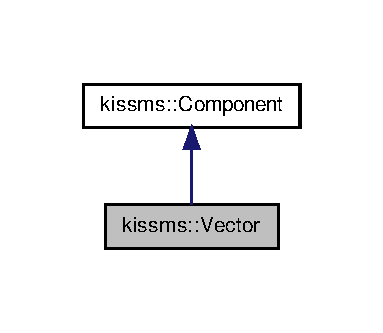
\includegraphics[width=184pt]{classkissms_1_1_vector__inherit__graph}
\end{center}
\end{figure}


Collaboration diagram for kissms\-:\-:Vector\-:
\nopagebreak
\begin{figure}[H]
\begin{center}
\leavevmode
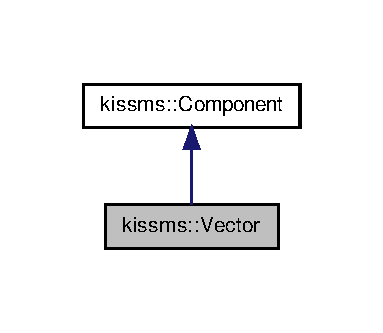
\includegraphics[width=184pt]{classkissms_1_1_vector__coll__graph}
\end{center}
\end{figure}
\subsection*{Additional Inherited Members}


\subsection{Detailed Description}


Definition at line 14 of file vector.\-h.



The documentation for this class was generated from the following file\-:\begin{DoxyCompactItemize}
\item 
/home/sieb/eclipse-\/workspace/eclipse-\/wrkspc\-\_\-\-F\-H/\-G\-D\-\_\-\-Phy\-Sim/src/kissms/component/vector-\/one/\hyperlink{vector_8h}{vector.\-h}\end{DoxyCompactItemize}

\hypertarget{classkissms_1_1_vectorproduct}{\section{kissms\-:\-:Vectorproduct Class Reference}
\label{classkissms_1_1_vectorproduct}\index{kissms\-::\-Vectorproduct@{kissms\-::\-Vectorproduct}}
}


{\ttfamily \#include $<$vectorproduct.\-h$>$}



Inheritance diagram for kissms\-:\-:Vectorproduct\-:
\nopagebreak
\begin{figure}[H]
\begin{center}
\leavevmode
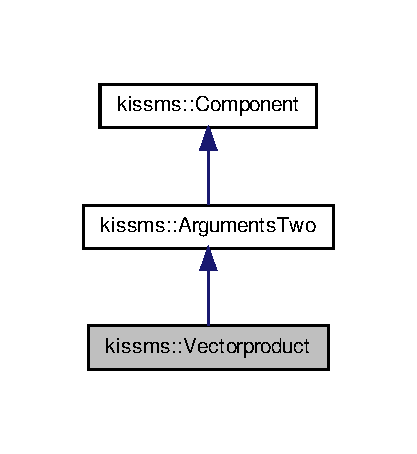
\includegraphics[width=200pt]{classkissms_1_1_vectorproduct__inherit__graph}
\end{center}
\end{figure}


Collaboration diagram for kissms\-:\-:Vectorproduct\-:
\nopagebreak
\begin{figure}[H]
\begin{center}
\leavevmode
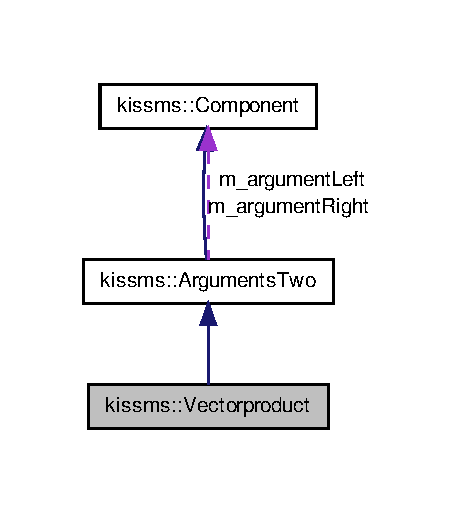
\includegraphics[width=218pt]{classkissms_1_1_vectorproduct__coll__graph}
\end{center}
\end{figure}
\subsection*{Additional Inherited Members}


\subsection{Detailed Description}


Definition at line 14 of file vectorproduct.\-h.



The documentation for this class was generated from the following file\-:\begin{DoxyCompactItemize}
\item 
/home/sieb/eclipse-\/workspace/eclipse-\/wrkspc\-\_\-\-F\-H/\-G\-D\-\_\-\-Phy\-Sim/src/kissms/component/vector-\/two/\hyperlink{vectorproduct_8h}{vectorproduct.\-h}\end{DoxyCompactItemize}

\chapter{File Documentation}
\hypertarget{arguments_one_8cpp}{\section{/home/sieb/eclipse-\/workspace/eclipse-\/wrkspc\-\_\-\-F\-H/\-G\-D\-\_\-\-Phy\-Sim/src/kissms/component/arguments\-One.cpp File Reference}
\label{arguments_one_8cpp}\index{/home/sieb/eclipse-\/workspace/eclipse-\/wrkspc\-\_\-\-F\-H/\-G\-D\-\_\-\-Phy\-Sim/src/kissms/component/arguments\-One.\-cpp@{/home/sieb/eclipse-\/workspace/eclipse-\/wrkspc\-\_\-\-F\-H/\-G\-D\-\_\-\-Phy\-Sim/src/kissms/component/arguments\-One.\-cpp}}
}
{\ttfamily \#include $<$kissms/kissms.\-h$>$}\\*
Include dependency graph for arguments\-One.\-cpp\-:
\nopagebreak
\begin{figure}[H]
\begin{center}
\leavevmode
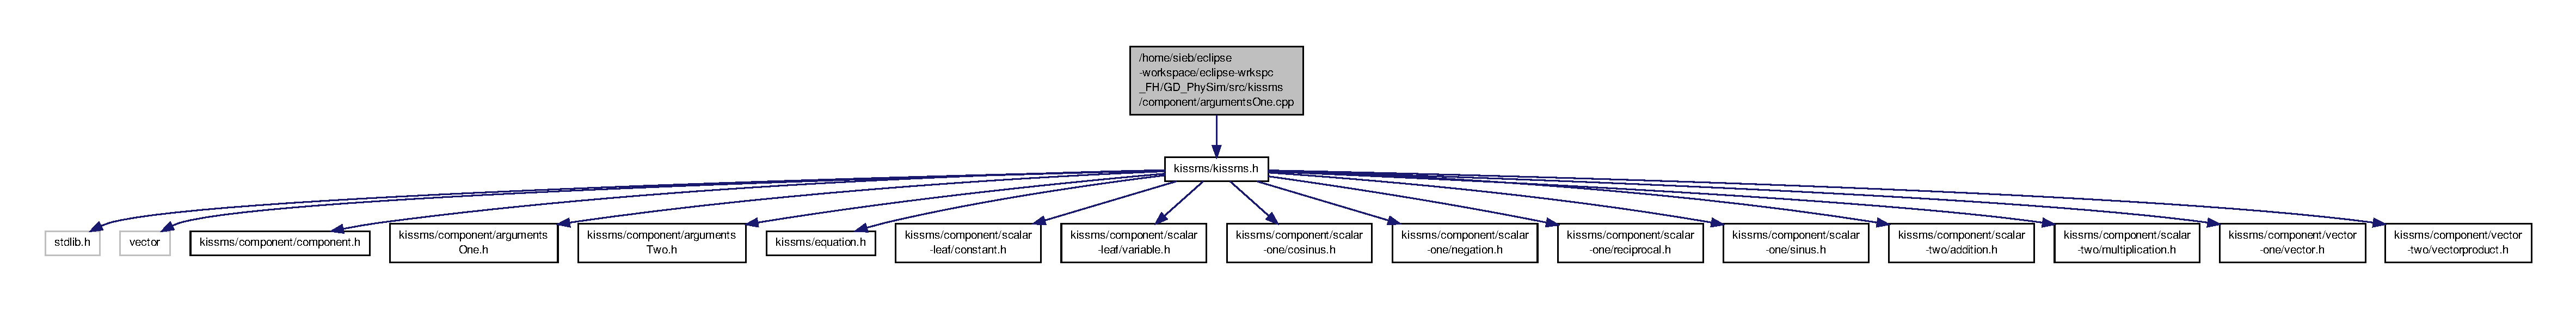
\includegraphics[width=350pt]{arguments_one_8cpp__incl}
\end{center}
\end{figure}
\subsection*{Namespaces}
\begin{DoxyCompactItemize}
\item 
\hyperlink{namespacekissms}{kissms}
\end{DoxyCompactItemize}
\subsection*{Constant Groups}
\begin{DoxyCompactItemize}
\item 
\hyperlink{namespacekissms}{kissms}
\end{DoxyCompactItemize}

\hypertarget{arguments_one_8h}{\section{/home/sieb/eclipse-\/workspace/eclipse-\/wrkspc\-\_\-\-F\-H/\-G\-D\-\_\-\-Phy\-Sim/src/kissms/component/arguments\-One.h File Reference}
\label{arguments_one_8h}\index{/home/sieb/eclipse-\/workspace/eclipse-\/wrkspc\-\_\-\-F\-H/\-G\-D\-\_\-\-Phy\-Sim/src/kissms/component/arguments\-One.\-h@{/home/sieb/eclipse-\/workspace/eclipse-\/wrkspc\-\_\-\-F\-H/\-G\-D\-\_\-\-Phy\-Sim/src/kissms/component/arguments\-One.\-h}}
}
This graph shows which files directly or indirectly include this file\-:
\nopagebreak
\begin{figure}[H]
\begin{center}
\leavevmode
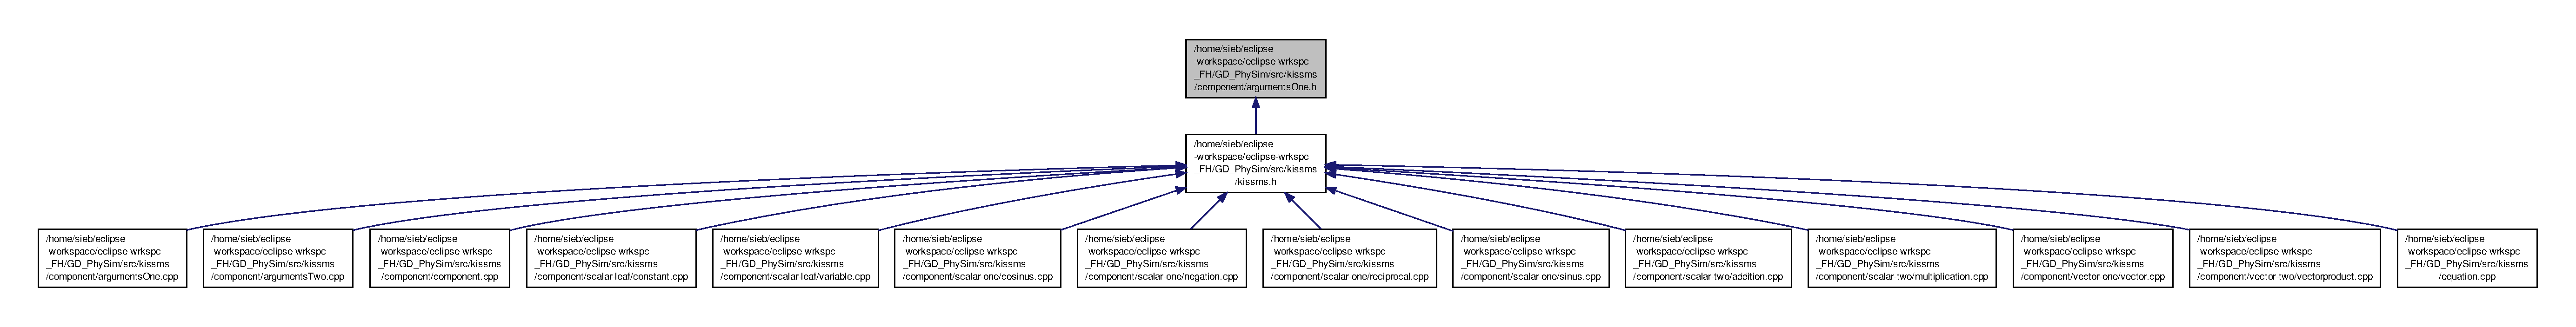
\includegraphics[width=350pt]{arguments_one_8h__dep__incl}
\end{center}
\end{figure}
\subsection*{Classes}
\begin{DoxyCompactItemize}
\item 
class \hyperlink{classkissms_1_1_arguments_one}{kissms\-::\-Arguments\-One}
\begin{DoxyCompactList}\small\item\em Representation of Components taking one argument. \end{DoxyCompactList}\end{DoxyCompactItemize}
\subsection*{Namespaces}
\begin{DoxyCompactItemize}
\item 
\hyperlink{namespacekissms}{kissms}
\end{DoxyCompactItemize}
\subsection*{Constant Groups}
\begin{DoxyCompactItemize}
\item 
\hyperlink{namespacekissms}{kissms}
\end{DoxyCompactItemize}

\hypertarget{arguments_two_8cpp}{\section{/home/sieb/eclipse-\/workspace/eclipse-\/wrkspc\-\_\-\-F\-H/\-G\-D\-\_\-\-Phy\-Sim/src/kissms/component/arguments\-Two.cpp File Reference}
\label{arguments_two_8cpp}\index{/home/sieb/eclipse-\/workspace/eclipse-\/wrkspc\-\_\-\-F\-H/\-G\-D\-\_\-\-Phy\-Sim/src/kissms/component/arguments\-Two.\-cpp@{/home/sieb/eclipse-\/workspace/eclipse-\/wrkspc\-\_\-\-F\-H/\-G\-D\-\_\-\-Phy\-Sim/src/kissms/component/arguments\-Two.\-cpp}}
}
{\ttfamily \#include $<$kissms/kissms.\-h$>$}\\*
Include dependency graph for arguments\-Two.\-cpp\-:
\nopagebreak
\begin{figure}[H]
\begin{center}
\leavevmode
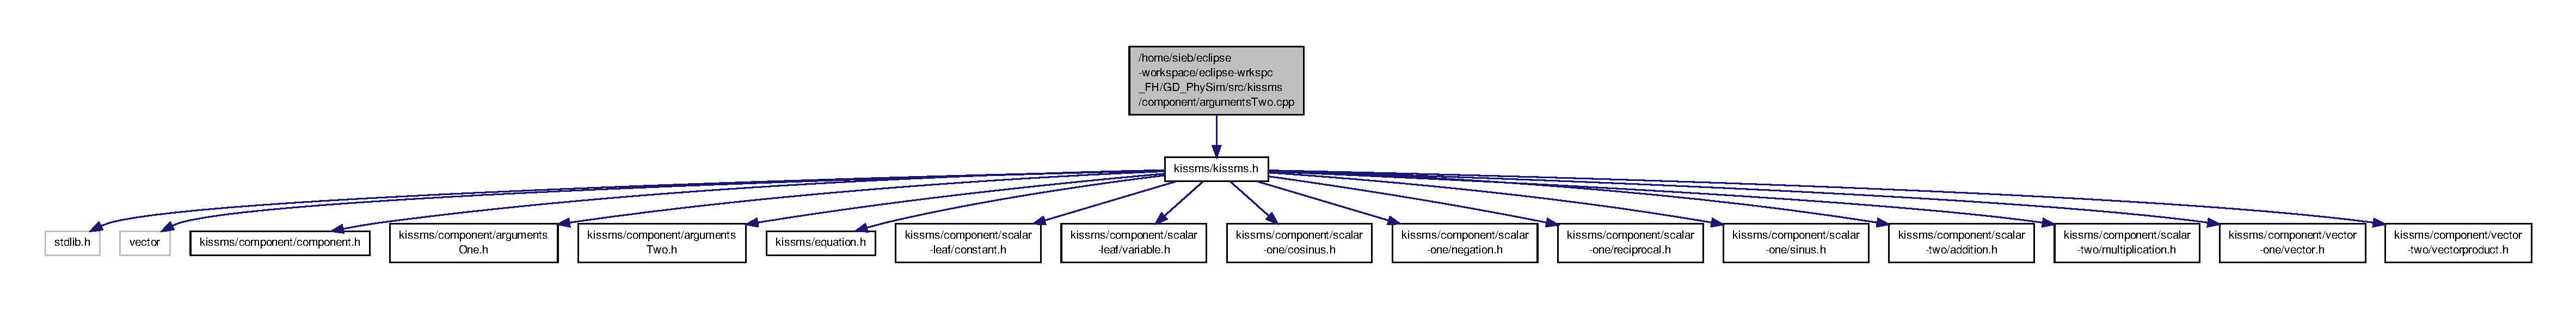
\includegraphics[width=350pt]{arguments_two_8cpp__incl}
\end{center}
\end{figure}
\subsection*{Namespaces}
\begin{DoxyCompactItemize}
\item 
\hyperlink{namespacekissms}{kissms}
\end{DoxyCompactItemize}
\subsection*{Constant Groups}
\begin{DoxyCompactItemize}
\item 
\hyperlink{namespacekissms}{kissms}
\end{DoxyCompactItemize}

\hypertarget{arguments_two_8h}{\section{/home/sieb/eclipse-\/workspace/eclipse-\/wrkspc\-\_\-\-F\-H/\-G\-D\-\_\-\-Phy\-Sim/src/kissms/component/arguments\-Two.h File Reference}
\label{arguments_two_8h}\index{/home/sieb/eclipse-\/workspace/eclipse-\/wrkspc\-\_\-\-F\-H/\-G\-D\-\_\-\-Phy\-Sim/src/kissms/component/arguments\-Two.\-h@{/home/sieb/eclipse-\/workspace/eclipse-\/wrkspc\-\_\-\-F\-H/\-G\-D\-\_\-\-Phy\-Sim/src/kissms/component/arguments\-Two.\-h}}
}
This graph shows which files directly or indirectly include this file\-:
\nopagebreak
\begin{figure}[H]
\begin{center}
\leavevmode
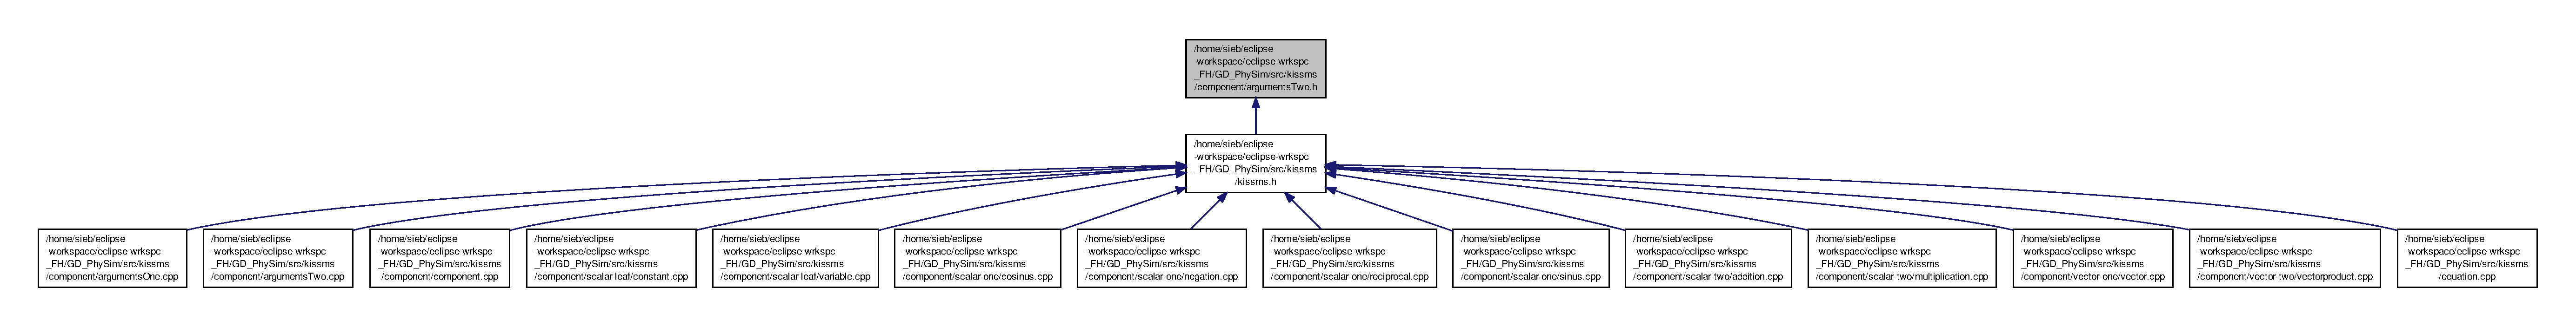
\includegraphics[width=350pt]{arguments_two_8h__dep__incl}
\end{center}
\end{figure}
\subsection*{Classes}
\begin{DoxyCompactItemize}
\item 
class \hyperlink{classkissms_1_1_arguments_two}{kissms\-::\-Arguments\-Two}
\begin{DoxyCompactList}\small\item\em Representation of Components taking two arguments. \end{DoxyCompactList}\end{DoxyCompactItemize}
\subsection*{Namespaces}
\begin{DoxyCompactItemize}
\item 
\hyperlink{namespacekissms}{kissms}
\end{DoxyCompactItemize}
\subsection*{Constant Groups}
\begin{DoxyCompactItemize}
\item 
\hyperlink{namespacekissms}{kissms}
\end{DoxyCompactItemize}

\hypertarget{component_8cpp}{\section{/home/sieb/eclipse-\/workspace/eclipse-\/wrkspc\-\_\-\-F\-H/\-G\-D\-\_\-\-Phy\-Sim/src/kissms/component/component.cpp File Reference}
\label{component_8cpp}\index{/home/sieb/eclipse-\/workspace/eclipse-\/wrkspc\-\_\-\-F\-H/\-G\-D\-\_\-\-Phy\-Sim/src/kissms/component/component.\-cpp@{/home/sieb/eclipse-\/workspace/eclipse-\/wrkspc\-\_\-\-F\-H/\-G\-D\-\_\-\-Phy\-Sim/src/kissms/component/component.\-cpp}}
}
{\ttfamily \#include $<$kissms/kissms.\-h$>$}\\*
Include dependency graph for component.\-cpp\-:
\nopagebreak
\begin{figure}[H]
\begin{center}
\leavevmode
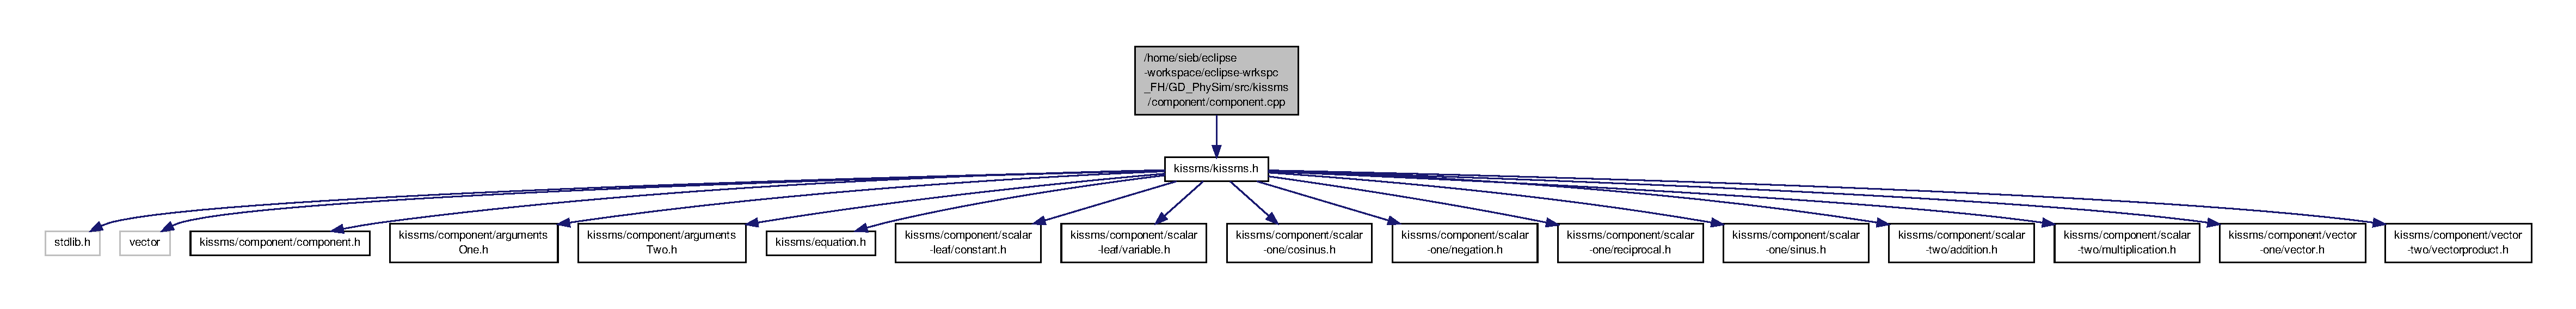
\includegraphics[width=350pt]{component_8cpp__incl}
\end{center}
\end{figure}
\subsection*{Namespaces}
\begin{DoxyCompactItemize}
\item 
\hyperlink{namespacekissms}{kissms}
\end{DoxyCompactItemize}
\subsection*{Constant Groups}
\begin{DoxyCompactItemize}
\item 
\hyperlink{namespacekissms}{kissms}
\end{DoxyCompactItemize}

\hypertarget{component_8h}{\section{/home/sieb/eclipse-\/workspace/eclipse-\/wrkspc\-\_\-\-F\-H/\-G\-D\-\_\-\-Phy\-Sim/src/kissms/component/component.h File Reference}
\label{component_8h}\index{/home/sieb/eclipse-\/workspace/eclipse-\/wrkspc\-\_\-\-F\-H/\-G\-D\-\_\-\-Phy\-Sim/src/kissms/component/component.\-h@{/home/sieb/eclipse-\/workspace/eclipse-\/wrkspc\-\_\-\-F\-H/\-G\-D\-\_\-\-Phy\-Sim/src/kissms/component/component.\-h}}
}
This graph shows which files directly or indirectly include this file\-:
\nopagebreak
\begin{figure}[H]
\begin{center}
\leavevmode
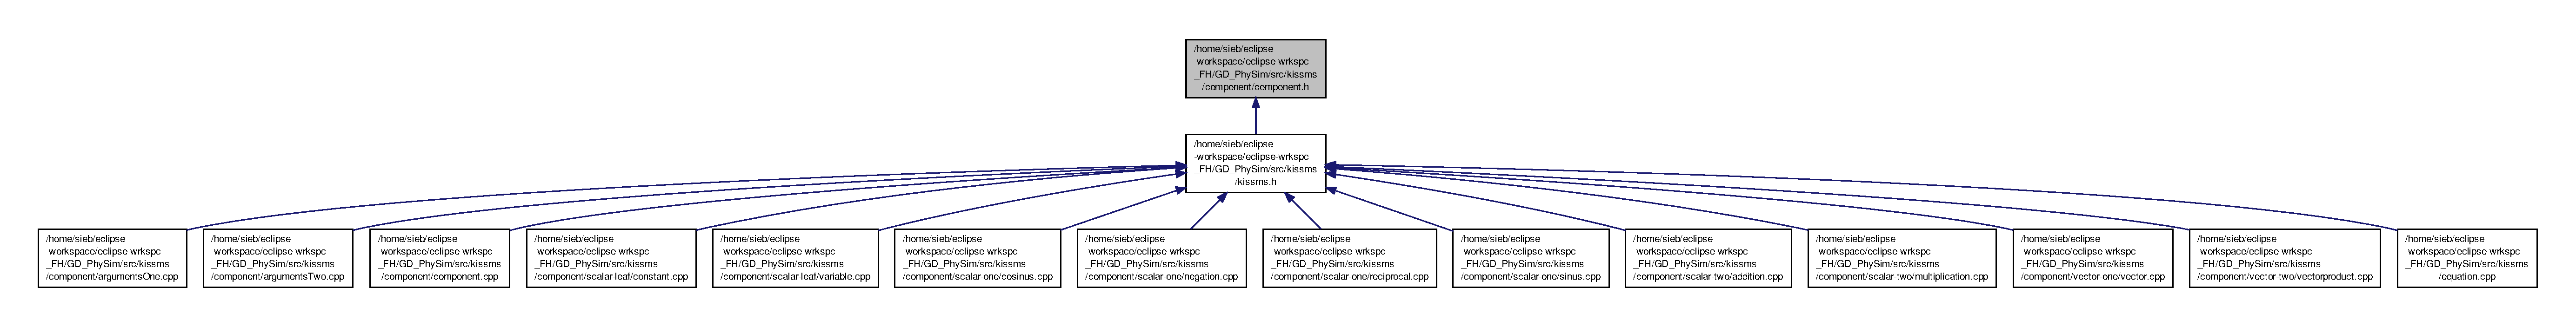
\includegraphics[width=350pt]{component_8h__dep__incl}
\end{center}
\end{figure}
\subsection*{Classes}
\begin{DoxyCompactItemize}
\item 
class \hyperlink{classkissms_1_1_component}{kissms\-::\-Component}
\begin{DoxyCompactList}\small\item\em Representation of a mathematical component in an \hyperlink{classkissms_1_1_equation}{Equation}. \end{DoxyCompactList}\end{DoxyCompactItemize}
\subsection*{Namespaces}
\begin{DoxyCompactItemize}
\item 
\hyperlink{namespacekissms}{kissms}
\end{DoxyCompactItemize}
\subsection*{Constant Groups}
\begin{DoxyCompactItemize}
\item 
\hyperlink{namespacekissms}{kissms}
\end{DoxyCompactItemize}

\hypertarget{constant_8cpp}{\section{/home/sieb/eclipse-\/workspace/eclipse-\/wrkspc\-\_\-\-F\-H/\-G\-D\-\_\-\-Phy\-Sim/src/kissms/component/scalar-\/leaf/constant.cpp File Reference}
\label{constant_8cpp}\index{/home/sieb/eclipse-\/workspace/eclipse-\/wrkspc\-\_\-\-F\-H/\-G\-D\-\_\-\-Phy\-Sim/src/kissms/component/scalar-\/leaf/constant.\-cpp@{/home/sieb/eclipse-\/workspace/eclipse-\/wrkspc\-\_\-\-F\-H/\-G\-D\-\_\-\-Phy\-Sim/src/kissms/component/scalar-\/leaf/constant.\-cpp}}
}
{\ttfamily \#include $<$kissms/kissms.\-h$>$}\\*
Include dependency graph for constant.\-cpp\-:
\nopagebreak
\begin{figure}[H]
\begin{center}
\leavevmode
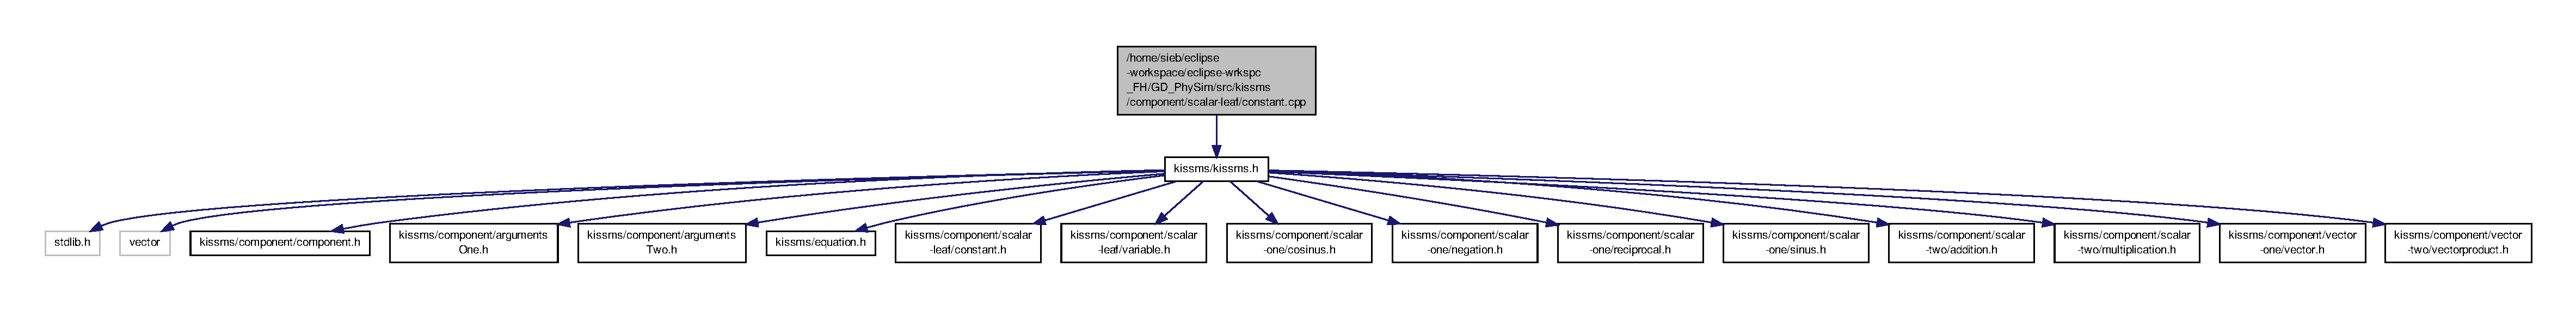
\includegraphics[width=350pt]{constant_8cpp__incl}
\end{center}
\end{figure}
\subsection*{Namespaces}
\begin{DoxyCompactItemize}
\item 
\hyperlink{namespacekissms}{kissms}
\end{DoxyCompactItemize}
\subsection*{Constant Groups}
\begin{DoxyCompactItemize}
\item 
\hyperlink{namespacekissms}{kissms}
\end{DoxyCompactItemize}

\hypertarget{constant_8h}{\section{/home/sieb/eclipse-\/workspace/eclipse-\/wrkspc\-\_\-\-F\-H/\-G\-D\-\_\-\-Phy\-Sim/src/kissms/component/scalar-\/leaf/constant.h File Reference}
\label{constant_8h}\index{/home/sieb/eclipse-\/workspace/eclipse-\/wrkspc\-\_\-\-F\-H/\-G\-D\-\_\-\-Phy\-Sim/src/kissms/component/scalar-\/leaf/constant.\-h@{/home/sieb/eclipse-\/workspace/eclipse-\/wrkspc\-\_\-\-F\-H/\-G\-D\-\_\-\-Phy\-Sim/src/kissms/component/scalar-\/leaf/constant.\-h}}
}
This graph shows which files directly or indirectly include this file\-:
\nopagebreak
\begin{figure}[H]
\begin{center}
\leavevmode
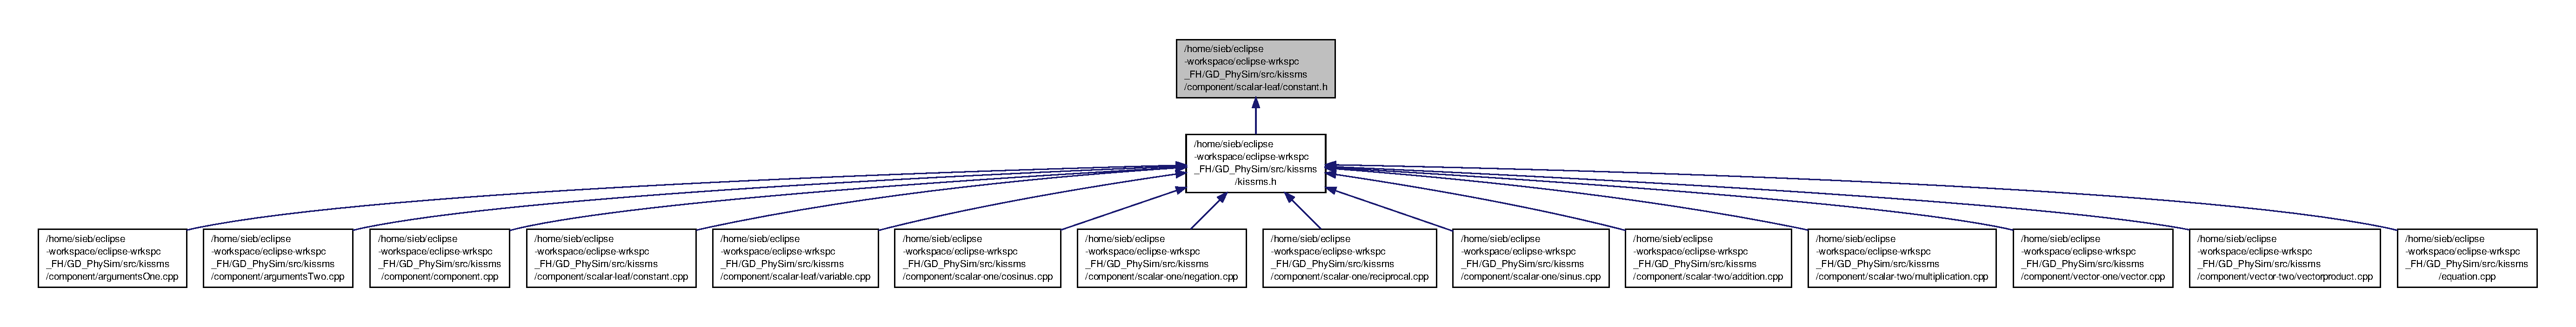
\includegraphics[width=350pt]{constant_8h__dep__incl}
\end{center}
\end{figure}
\subsection*{Classes}
\begin{DoxyCompactItemize}
\item 
class \hyperlink{classkissms_1_1_constant}{kissms\-::\-Constant}
\end{DoxyCompactItemize}
\subsection*{Namespaces}
\begin{DoxyCompactItemize}
\item 
\hyperlink{namespacekissms}{kissms}
\end{DoxyCompactItemize}
\subsection*{Constant Groups}
\begin{DoxyCompactItemize}
\item 
\hyperlink{namespacekissms}{kissms}
\end{DoxyCompactItemize}

\hypertarget{variable_8cpp}{\section{/home/sieb/eclipse-\/workspace/eclipse-\/wrkspc\-\_\-\-F\-H/\-G\-D\-\_\-\-Phy\-Sim/src/kissms/component/scalar-\/leaf/variable.cpp File Reference}
\label{variable_8cpp}\index{/home/sieb/eclipse-\/workspace/eclipse-\/wrkspc\-\_\-\-F\-H/\-G\-D\-\_\-\-Phy\-Sim/src/kissms/component/scalar-\/leaf/variable.\-cpp@{/home/sieb/eclipse-\/workspace/eclipse-\/wrkspc\-\_\-\-F\-H/\-G\-D\-\_\-\-Phy\-Sim/src/kissms/component/scalar-\/leaf/variable.\-cpp}}
}
{\ttfamily \#include $<$kissms/kissms.\-h$>$}\\*
Include dependency graph for variable.\-cpp\-:
\nopagebreak
\begin{figure}[H]
\begin{center}
\leavevmode
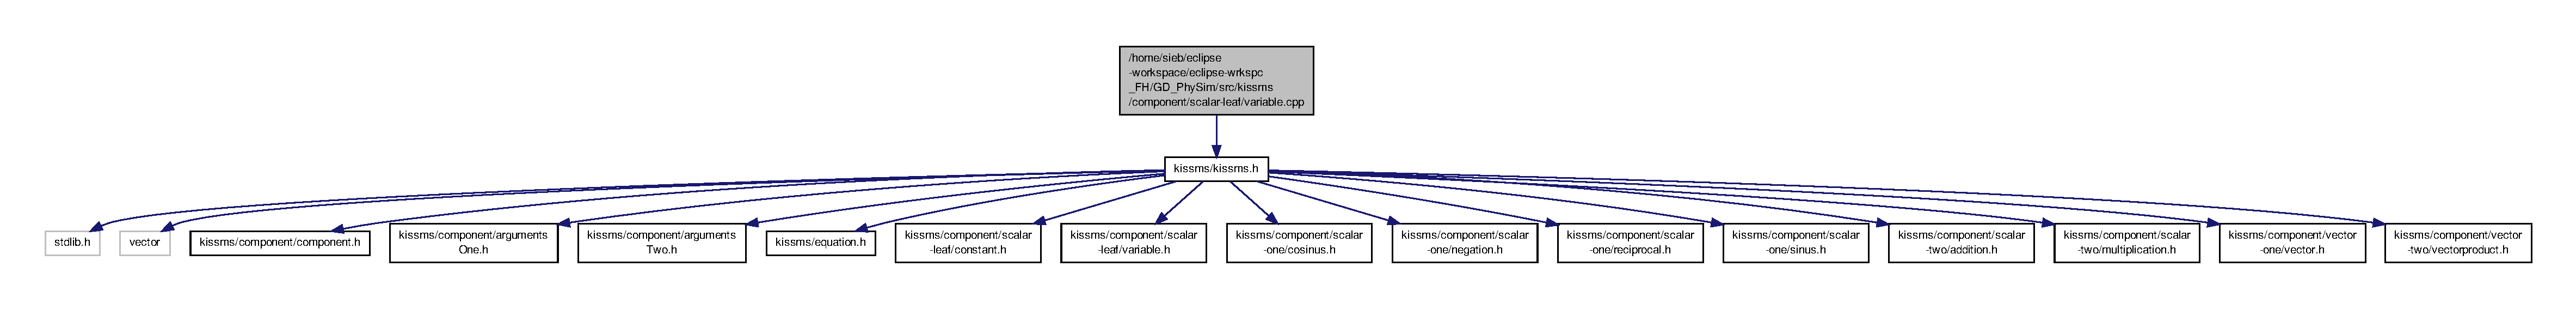
\includegraphics[width=350pt]{variable_8cpp__incl}
\end{center}
\end{figure}
\subsection*{Namespaces}
\begin{DoxyCompactItemize}
\item 
\hyperlink{namespacekissms}{kissms}
\end{DoxyCompactItemize}
\subsection*{Constant Groups}
\begin{DoxyCompactItemize}
\item 
\hyperlink{namespacekissms}{kissms}
\end{DoxyCompactItemize}

\hypertarget{variable_8h}{\section{/home/sieb/eclipse-\/workspace/eclipse-\/wrkspc\-\_\-\-F\-H/\-G\-D\-\_\-\-Phy\-Sim/src/kissms/component/scalar-\/leaf/variable.h File Reference}
\label{variable_8h}\index{/home/sieb/eclipse-\/workspace/eclipse-\/wrkspc\-\_\-\-F\-H/\-G\-D\-\_\-\-Phy\-Sim/src/kissms/component/scalar-\/leaf/variable.\-h@{/home/sieb/eclipse-\/workspace/eclipse-\/wrkspc\-\_\-\-F\-H/\-G\-D\-\_\-\-Phy\-Sim/src/kissms/component/scalar-\/leaf/variable.\-h}}
}
This graph shows which files directly or indirectly include this file\-:
\nopagebreak
\begin{figure}[H]
\begin{center}
\leavevmode
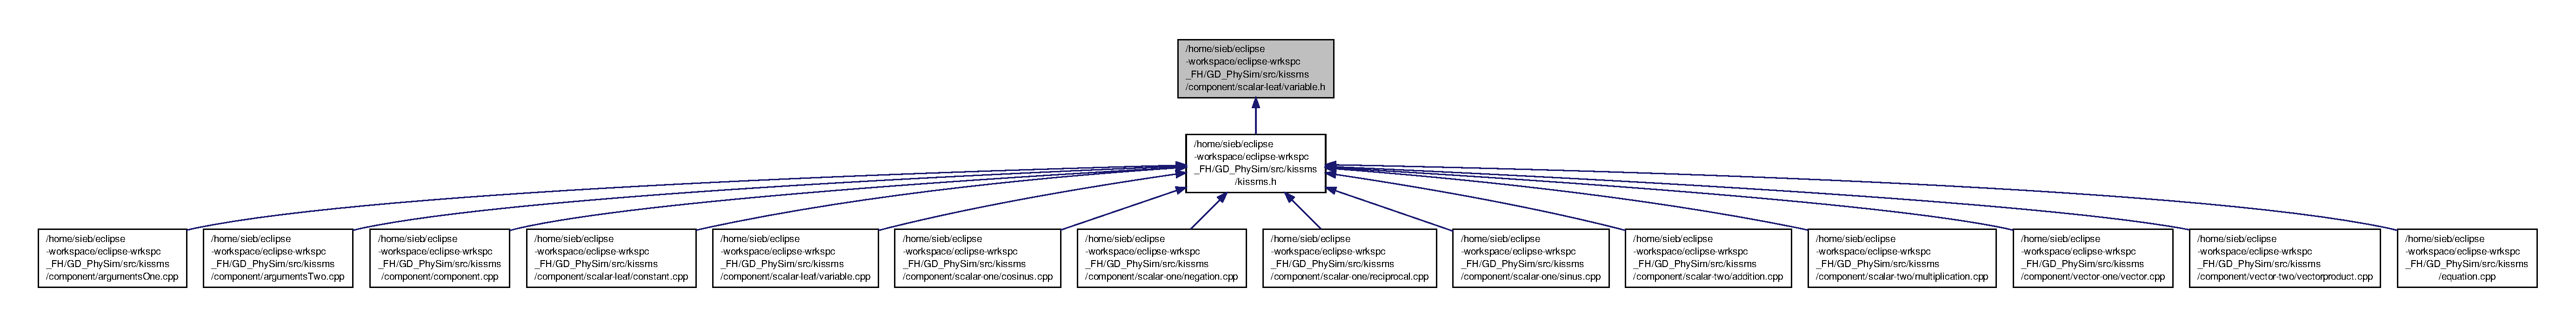
\includegraphics[width=350pt]{variable_8h__dep__incl}
\end{center}
\end{figure}
\subsection*{Classes}
\begin{DoxyCompactItemize}
\item 
class \hyperlink{classkissms_1_1_variable}{kissms\-::\-Variable}
\begin{DoxyCompactList}\small\item\em \hyperlink{classkissms_1_1_component}{Component} representing a single variable value. \end{DoxyCompactList}\end{DoxyCompactItemize}
\subsection*{Namespaces}
\begin{DoxyCompactItemize}
\item 
\hyperlink{namespacekissms}{kissms}
\end{DoxyCompactItemize}
\subsection*{Constant Groups}
\begin{DoxyCompactItemize}
\item 
\hyperlink{namespacekissms}{kissms}
\end{DoxyCompactItemize}

\hypertarget{cosinus_8cpp}{\section{/home/sieb/eclipse-\/workspace/eclipse-\/wrkspc\-\_\-\-F\-H/\-G\-D\-\_\-\-Phy\-Sim/src/kissms/component/scalar-\/one/cosinus.cpp File Reference}
\label{cosinus_8cpp}\index{/home/sieb/eclipse-\/workspace/eclipse-\/wrkspc\-\_\-\-F\-H/\-G\-D\-\_\-\-Phy\-Sim/src/kissms/component/scalar-\/one/cosinus.\-cpp@{/home/sieb/eclipse-\/workspace/eclipse-\/wrkspc\-\_\-\-F\-H/\-G\-D\-\_\-\-Phy\-Sim/src/kissms/component/scalar-\/one/cosinus.\-cpp}}
}
{\ttfamily \#include $<$kissms/kissms.\-h$>$}\\*
Include dependency graph for cosinus.\-cpp\-:
\nopagebreak
\begin{figure}[H]
\begin{center}
\leavevmode
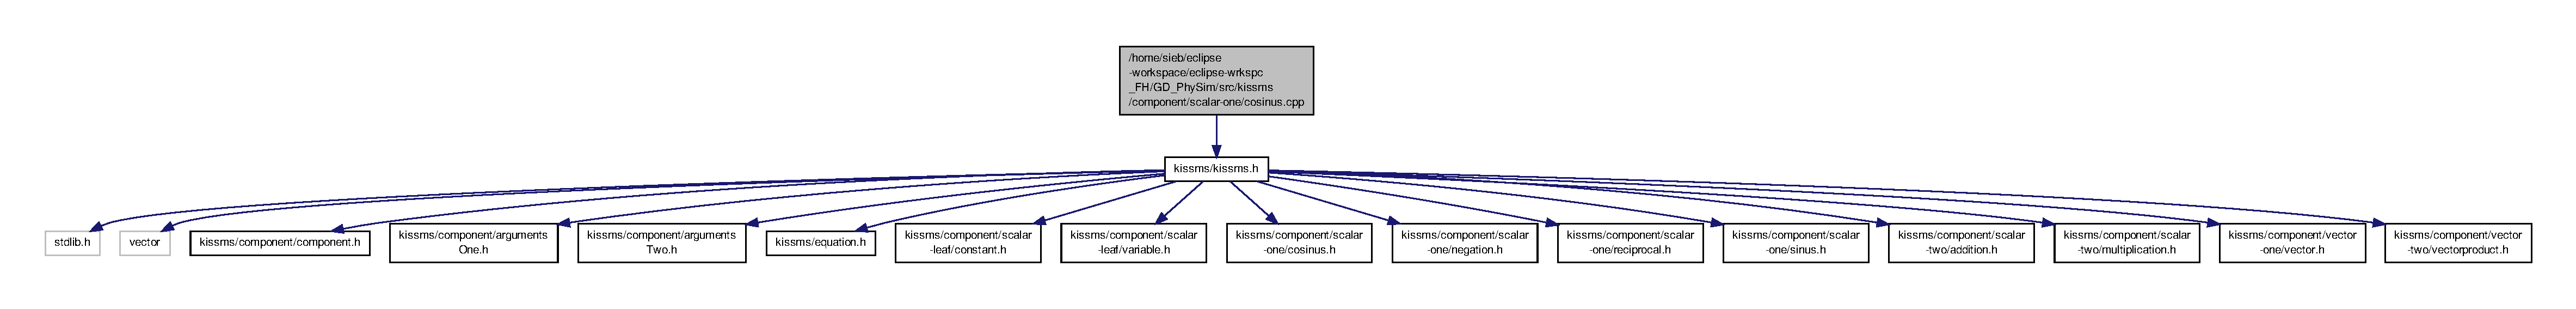
\includegraphics[width=350pt]{cosinus_8cpp__incl}
\end{center}
\end{figure}
\subsection*{Namespaces}
\begin{DoxyCompactItemize}
\item 
\hyperlink{namespacekissms}{kissms}
\end{DoxyCompactItemize}
\subsection*{Constant Groups}
\begin{DoxyCompactItemize}
\item 
\hyperlink{namespacekissms}{kissms}
\end{DoxyCompactItemize}

\hypertarget{cosinus_8h}{\section{/home/sieb/eclipse-\/workspace/eclipse-\/wrkspc\-\_\-\-F\-H/\-G\-D\-\_\-\-Phy\-Sim/src/kissms/component/scalar-\/one/cosinus.h File Reference}
\label{cosinus_8h}\index{/home/sieb/eclipse-\/workspace/eclipse-\/wrkspc\-\_\-\-F\-H/\-G\-D\-\_\-\-Phy\-Sim/src/kissms/component/scalar-\/one/cosinus.\-h@{/home/sieb/eclipse-\/workspace/eclipse-\/wrkspc\-\_\-\-F\-H/\-G\-D\-\_\-\-Phy\-Sim/src/kissms/component/scalar-\/one/cosinus.\-h}}
}
This graph shows which files directly or indirectly include this file\-:
\nopagebreak
\begin{figure}[H]
\begin{center}
\leavevmode
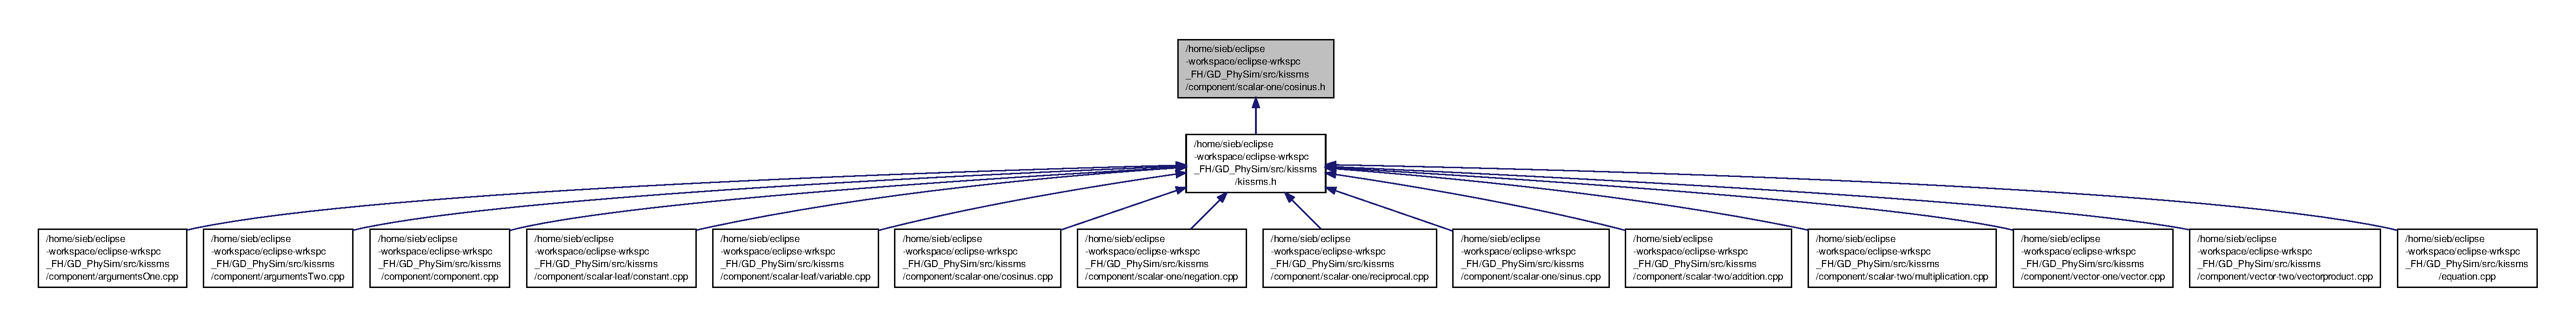
\includegraphics[width=350pt]{cosinus_8h__dep__incl}
\end{center}
\end{figure}
\subsection*{Classes}
\begin{DoxyCompactItemize}
\item 
class \hyperlink{classkissms_1_1_cosinus}{kissms\-::\-Cosinus}
\end{DoxyCompactItemize}
\subsection*{Namespaces}
\begin{DoxyCompactItemize}
\item 
\hyperlink{namespacekissms}{kissms}
\end{DoxyCompactItemize}
\subsection*{Constant Groups}
\begin{DoxyCompactItemize}
\item 
\hyperlink{namespacekissms}{kissms}
\end{DoxyCompactItemize}

\hypertarget{negation_8cpp}{\section{/home/sieb/eclipse-\/workspace/eclipse-\/wrkspc\-\_\-\-F\-H/\-G\-D\-\_\-\-Phy\-Sim/src/kissms/component/scalar-\/one/negation.cpp File Reference}
\label{negation_8cpp}\index{/home/sieb/eclipse-\/workspace/eclipse-\/wrkspc\-\_\-\-F\-H/\-G\-D\-\_\-\-Phy\-Sim/src/kissms/component/scalar-\/one/negation.\-cpp@{/home/sieb/eclipse-\/workspace/eclipse-\/wrkspc\-\_\-\-F\-H/\-G\-D\-\_\-\-Phy\-Sim/src/kissms/component/scalar-\/one/negation.\-cpp}}
}
{\ttfamily \#include $<$kissms/kissms.\-h$>$}\\*
Include dependency graph for negation.\-cpp\-:
\nopagebreak
\begin{figure}[H]
\begin{center}
\leavevmode
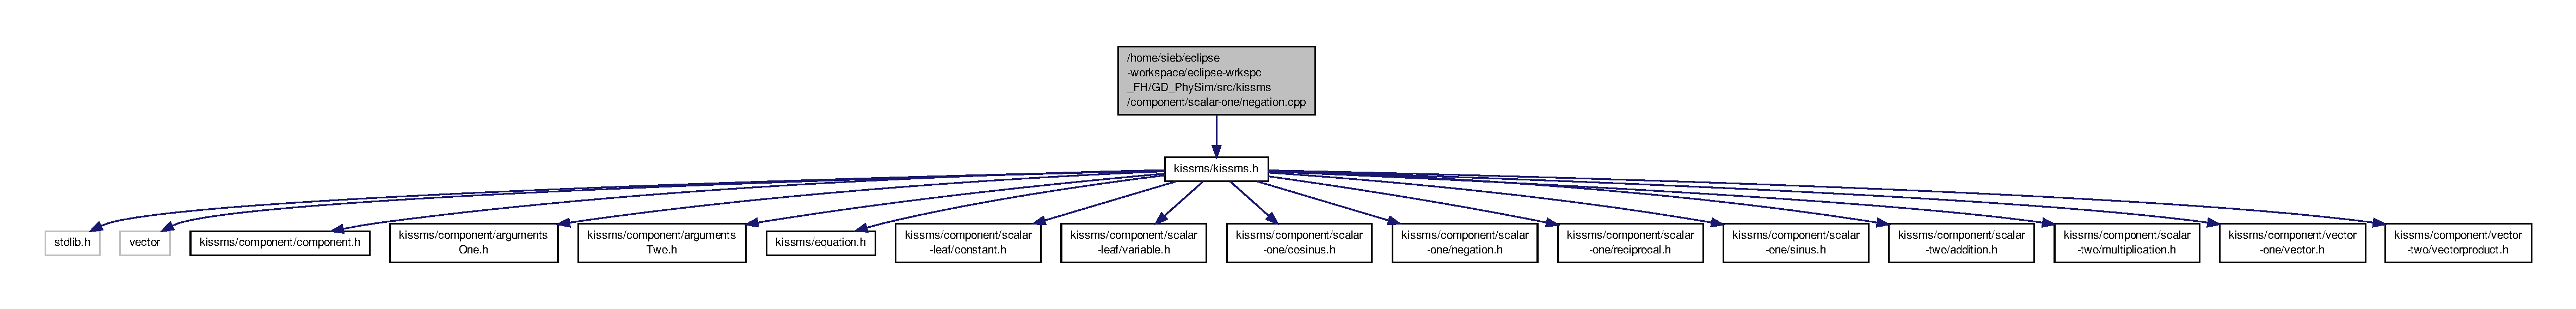
\includegraphics[width=350pt]{negation_8cpp__incl}
\end{center}
\end{figure}
\subsection*{Namespaces}
\begin{DoxyCompactItemize}
\item 
\hyperlink{namespacekissms}{kissms}
\end{DoxyCompactItemize}
\subsection*{Constant Groups}
\begin{DoxyCompactItemize}
\item 
\hyperlink{namespacekissms}{kissms}
\end{DoxyCompactItemize}

\hypertarget{negation_8h}{\section{/home/sieb/eclipse-\/workspace/eclipse-\/wrkspc\-\_\-\-F\-H/\-G\-D\-\_\-\-Phy\-Sim/src/kissms/component/scalar-\/one/negation.h File Reference}
\label{negation_8h}\index{/home/sieb/eclipse-\/workspace/eclipse-\/wrkspc\-\_\-\-F\-H/\-G\-D\-\_\-\-Phy\-Sim/src/kissms/component/scalar-\/one/negation.\-h@{/home/sieb/eclipse-\/workspace/eclipse-\/wrkspc\-\_\-\-F\-H/\-G\-D\-\_\-\-Phy\-Sim/src/kissms/component/scalar-\/one/negation.\-h}}
}
This graph shows which files directly or indirectly include this file\-:
\nopagebreak
\begin{figure}[H]
\begin{center}
\leavevmode
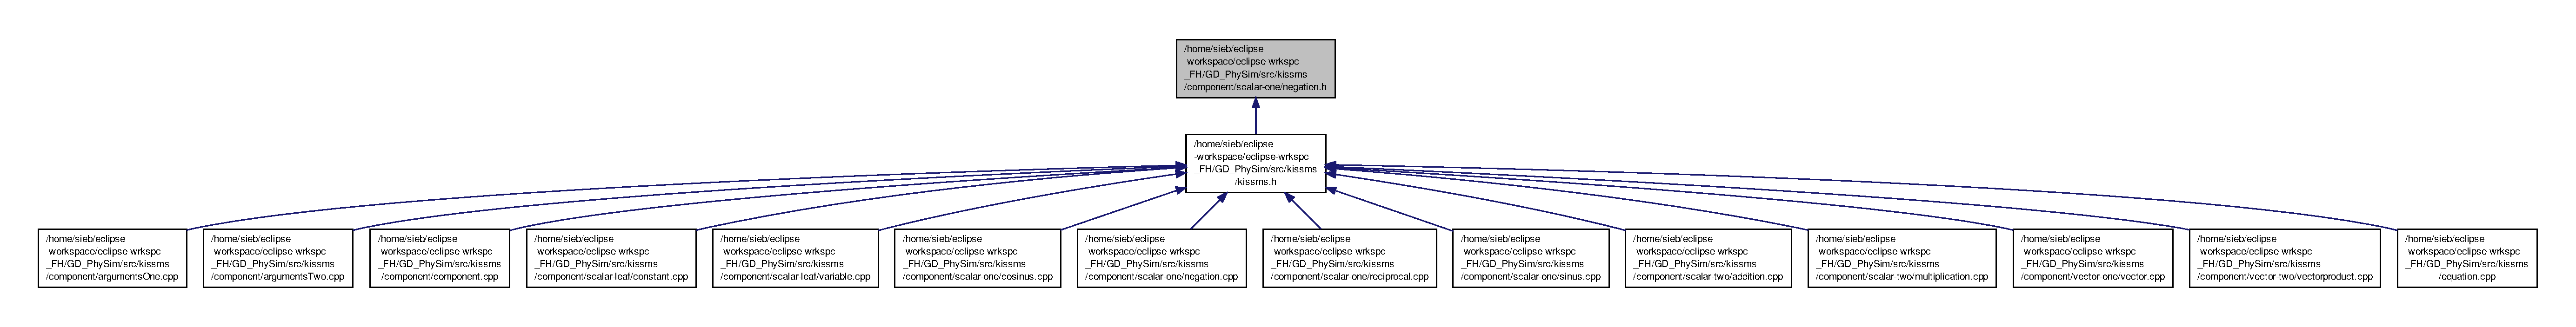
\includegraphics[width=350pt]{negation_8h__dep__incl}
\end{center}
\end{figure}
\subsection*{Classes}
\begin{DoxyCompactItemize}
\item 
class \hyperlink{classkissms_1_1_negation}{kissms\-::\-Negation}
\end{DoxyCompactItemize}
\subsection*{Namespaces}
\begin{DoxyCompactItemize}
\item 
\hyperlink{namespacekissms}{kissms}
\end{DoxyCompactItemize}
\subsection*{Constant Groups}
\begin{DoxyCompactItemize}
\item 
\hyperlink{namespacekissms}{kissms}
\end{DoxyCompactItemize}

\hypertarget{reciprocal_8cpp}{\section{/home/sieb/eclipse-\/workspace/eclipse-\/wrkspc\-\_\-\-F\-H/\-G\-D\-\_\-\-Phy\-Sim/src/kissms/component/scalar-\/one/reciprocal.cpp File Reference}
\label{reciprocal_8cpp}\index{/home/sieb/eclipse-\/workspace/eclipse-\/wrkspc\-\_\-\-F\-H/\-G\-D\-\_\-\-Phy\-Sim/src/kissms/component/scalar-\/one/reciprocal.\-cpp@{/home/sieb/eclipse-\/workspace/eclipse-\/wrkspc\-\_\-\-F\-H/\-G\-D\-\_\-\-Phy\-Sim/src/kissms/component/scalar-\/one/reciprocal.\-cpp}}
}
{\ttfamily \#include $<$kissms/kissms.\-h$>$}\\*
Include dependency graph for reciprocal.\-cpp\-:
\nopagebreak
\begin{figure}[H]
\begin{center}
\leavevmode
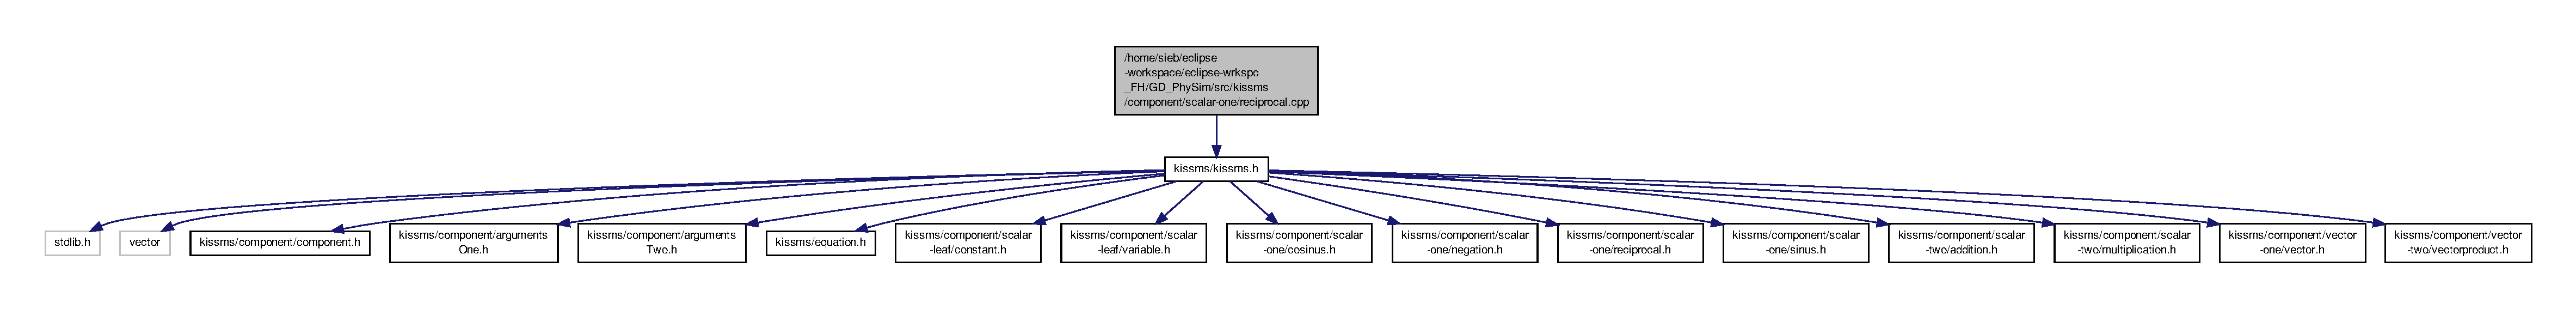
\includegraphics[width=350pt]{reciprocal_8cpp__incl}
\end{center}
\end{figure}
\subsection*{Namespaces}
\begin{DoxyCompactItemize}
\item 
\hyperlink{namespacekissms}{kissms}
\end{DoxyCompactItemize}
\subsection*{Constant Groups}
\begin{DoxyCompactItemize}
\item 
\hyperlink{namespacekissms}{kissms}
\end{DoxyCompactItemize}

\hypertarget{reciprocal_8h}{\section{/home/sieb/eclipse-\/workspace/eclipse-\/wrkspc\-\_\-\-F\-H/\-G\-D\-\_\-\-Phy\-Sim/src/kissms/component/scalar-\/one/reciprocal.h File Reference}
\label{reciprocal_8h}\index{/home/sieb/eclipse-\/workspace/eclipse-\/wrkspc\-\_\-\-F\-H/\-G\-D\-\_\-\-Phy\-Sim/src/kissms/component/scalar-\/one/reciprocal.\-h@{/home/sieb/eclipse-\/workspace/eclipse-\/wrkspc\-\_\-\-F\-H/\-G\-D\-\_\-\-Phy\-Sim/src/kissms/component/scalar-\/one/reciprocal.\-h}}
}
This graph shows which files directly or indirectly include this file\-:
\nopagebreak
\begin{figure}[H]
\begin{center}
\leavevmode
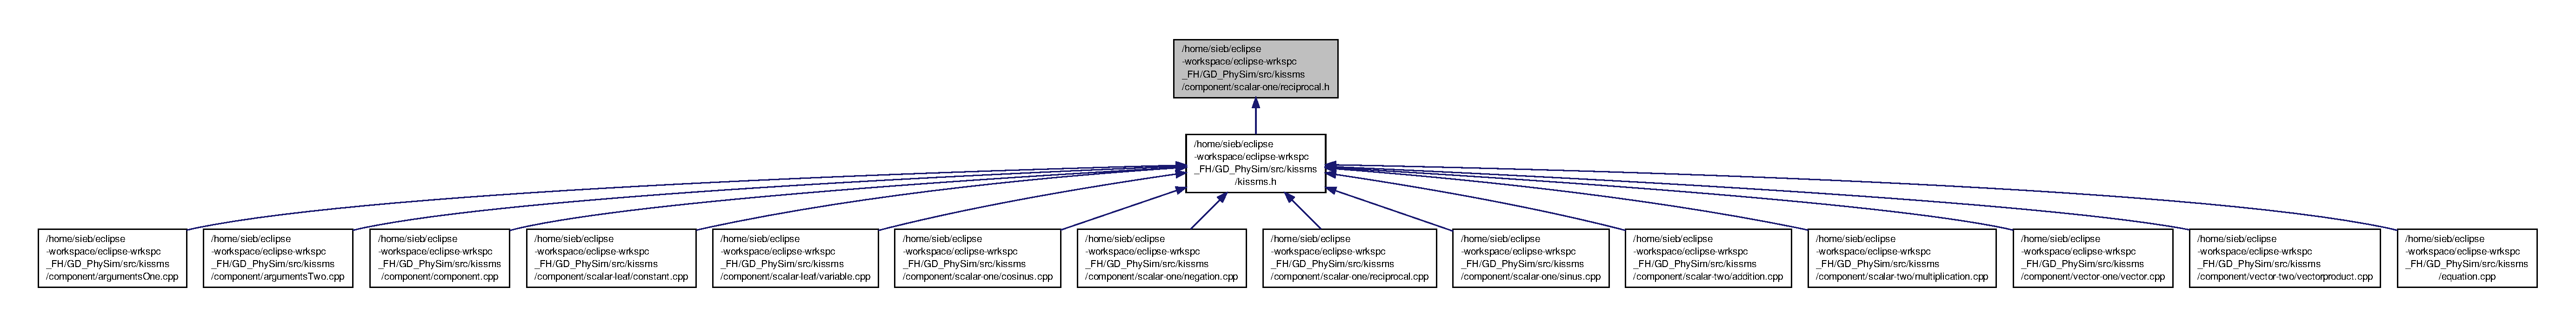
\includegraphics[width=350pt]{reciprocal_8h__dep__incl}
\end{center}
\end{figure}
\subsection*{Classes}
\begin{DoxyCompactItemize}
\item 
class \hyperlink{classkissms_1_1_reciprocal}{kissms\-::\-Reciprocal}
\end{DoxyCompactItemize}
\subsection*{Namespaces}
\begin{DoxyCompactItemize}
\item 
\hyperlink{namespacekissms}{kissms}
\end{DoxyCompactItemize}
\subsection*{Constant Groups}
\begin{DoxyCompactItemize}
\item 
\hyperlink{namespacekissms}{kissms}
\end{DoxyCompactItemize}

\hypertarget{sinus_8cpp}{\section{/home/sieb/eclipse-\/workspace/eclipse-\/wrkspc\-\_\-\-F\-H/\-G\-D\-\_\-\-Phy\-Sim/src/kissms/component/scalar-\/one/sinus.cpp File Reference}
\label{sinus_8cpp}\index{/home/sieb/eclipse-\/workspace/eclipse-\/wrkspc\-\_\-\-F\-H/\-G\-D\-\_\-\-Phy\-Sim/src/kissms/component/scalar-\/one/sinus.\-cpp@{/home/sieb/eclipse-\/workspace/eclipse-\/wrkspc\-\_\-\-F\-H/\-G\-D\-\_\-\-Phy\-Sim/src/kissms/component/scalar-\/one/sinus.\-cpp}}
}
{\ttfamily \#include $<$kissms/kissms.\-h$>$}\\*
Include dependency graph for sinus.\-cpp\-:
\nopagebreak
\begin{figure}[H]
\begin{center}
\leavevmode
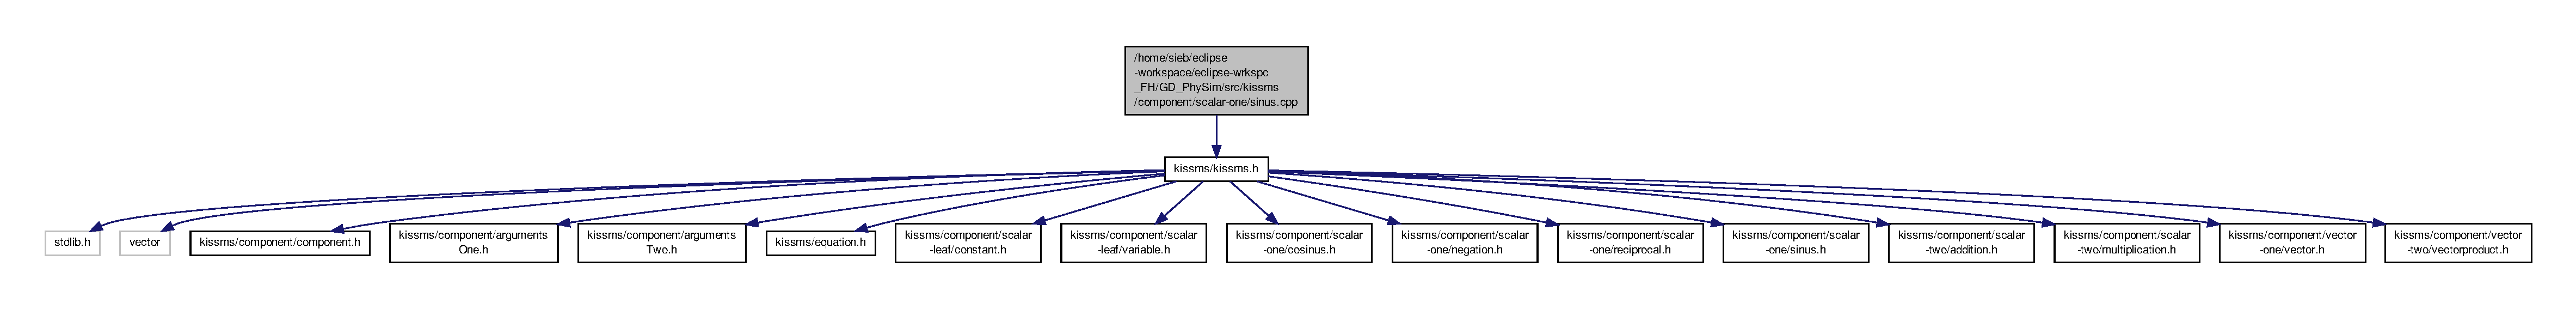
\includegraphics[width=350pt]{sinus_8cpp__incl}
\end{center}
\end{figure}
\subsection*{Namespaces}
\begin{DoxyCompactItemize}
\item 
\hyperlink{namespacekissms}{kissms}
\end{DoxyCompactItemize}
\subsection*{Constant Groups}
\begin{DoxyCompactItemize}
\item 
\hyperlink{namespacekissms}{kissms}
\end{DoxyCompactItemize}

\hypertarget{sinus_8h}{\section{/home/sieb/eclipse-\/workspace/eclipse-\/wrkspc\-\_\-\-F\-H/\-G\-D\-\_\-\-Phy\-Sim/src/kissms/component/scalar-\/one/sinus.h File Reference}
\label{sinus_8h}\index{/home/sieb/eclipse-\/workspace/eclipse-\/wrkspc\-\_\-\-F\-H/\-G\-D\-\_\-\-Phy\-Sim/src/kissms/component/scalar-\/one/sinus.\-h@{/home/sieb/eclipse-\/workspace/eclipse-\/wrkspc\-\_\-\-F\-H/\-G\-D\-\_\-\-Phy\-Sim/src/kissms/component/scalar-\/one/sinus.\-h}}
}
This graph shows which files directly or indirectly include this file\-:
\nopagebreak
\begin{figure}[H]
\begin{center}
\leavevmode
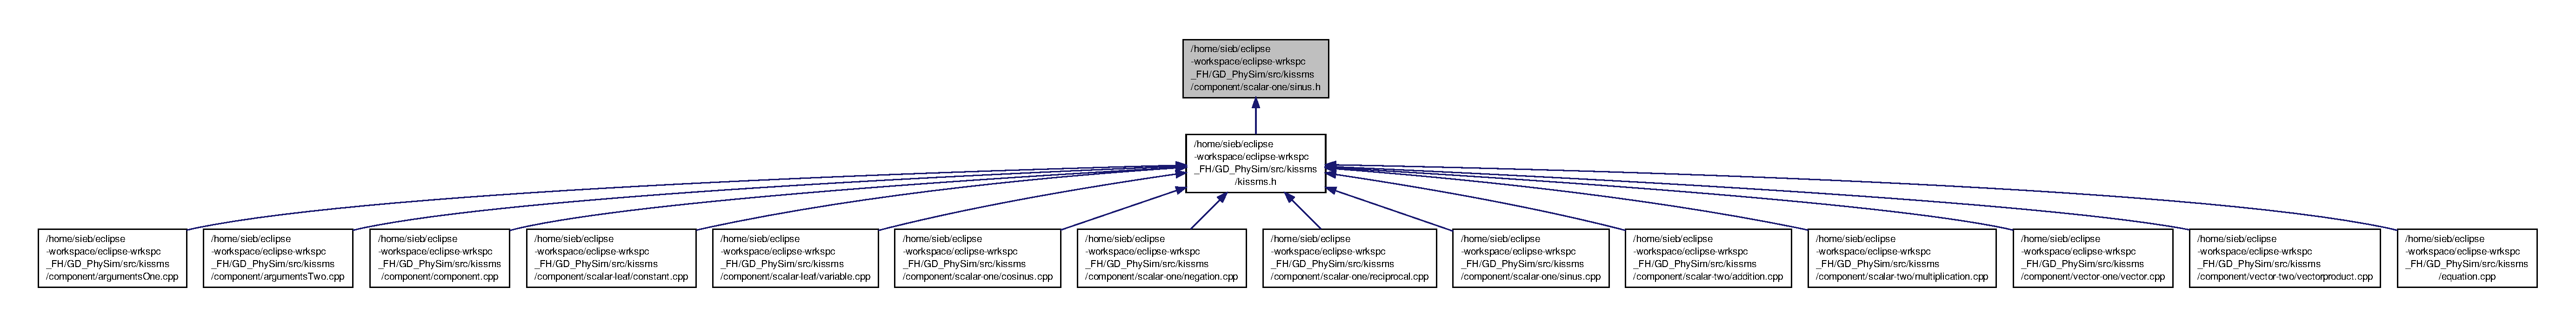
\includegraphics[width=350pt]{sinus_8h__dep__incl}
\end{center}
\end{figure}
\subsection*{Classes}
\begin{DoxyCompactItemize}
\item 
class \hyperlink{classkissms_1_1_sinus}{kissms\-::\-Sinus}
\end{DoxyCompactItemize}
\subsection*{Namespaces}
\begin{DoxyCompactItemize}
\item 
\hyperlink{namespacekissms}{kissms}
\end{DoxyCompactItemize}
\subsection*{Constant Groups}
\begin{DoxyCompactItemize}
\item 
\hyperlink{namespacekissms}{kissms}
\end{DoxyCompactItemize}

\hypertarget{addition_8cpp}{\section{/home/sieb/eclipse-\/workspace/eclipse-\/wrkspc\-\_\-\-F\-H/\-G\-D\-\_\-\-Phy\-Sim/src/kissms/component/scalar-\/two/addition.cpp File Reference}
\label{addition_8cpp}\index{/home/sieb/eclipse-\/workspace/eclipse-\/wrkspc\-\_\-\-F\-H/\-G\-D\-\_\-\-Phy\-Sim/src/kissms/component/scalar-\/two/addition.\-cpp@{/home/sieb/eclipse-\/workspace/eclipse-\/wrkspc\-\_\-\-F\-H/\-G\-D\-\_\-\-Phy\-Sim/src/kissms/component/scalar-\/two/addition.\-cpp}}
}
{\ttfamily \#include $<$kissms/kissms.\-h$>$}\\*
Include dependency graph for addition.\-cpp\-:
\nopagebreak
\begin{figure}[H]
\begin{center}
\leavevmode
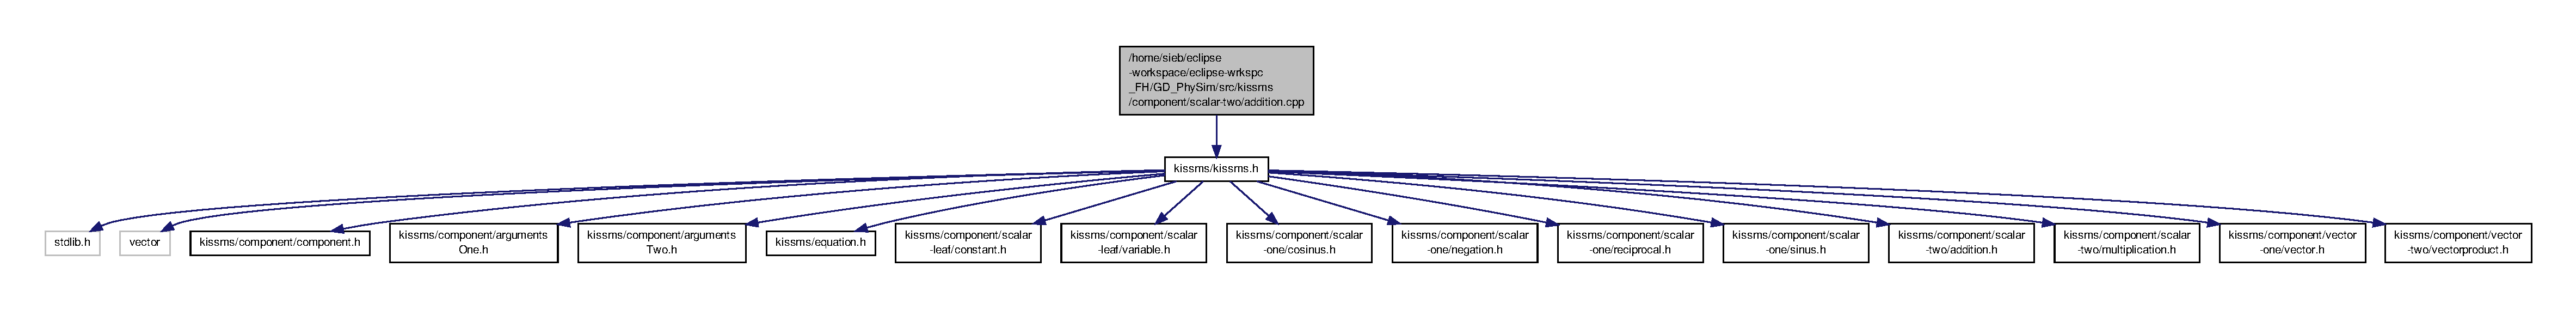
\includegraphics[width=350pt]{addition_8cpp__incl}
\end{center}
\end{figure}
\subsection*{Namespaces}
\begin{DoxyCompactItemize}
\item 
\hyperlink{namespacekissms}{kissms}
\end{DoxyCompactItemize}
\subsection*{Constant Groups}
\begin{DoxyCompactItemize}
\item 
\hyperlink{namespacekissms}{kissms}
\end{DoxyCompactItemize}

\hypertarget{addition_8h}{\section{/home/sieb/eclipse-\/workspace/eclipse-\/wrkspc\-\_\-\-F\-H/\-G\-D\-\_\-\-Phy\-Sim/src/kissms/component/scalar-\/two/addition.h File Reference}
\label{addition_8h}\index{/home/sieb/eclipse-\/workspace/eclipse-\/wrkspc\-\_\-\-F\-H/\-G\-D\-\_\-\-Phy\-Sim/src/kissms/component/scalar-\/two/addition.\-h@{/home/sieb/eclipse-\/workspace/eclipse-\/wrkspc\-\_\-\-F\-H/\-G\-D\-\_\-\-Phy\-Sim/src/kissms/component/scalar-\/two/addition.\-h}}
}
This graph shows which files directly or indirectly include this file\-:
\nopagebreak
\begin{figure}[H]
\begin{center}
\leavevmode
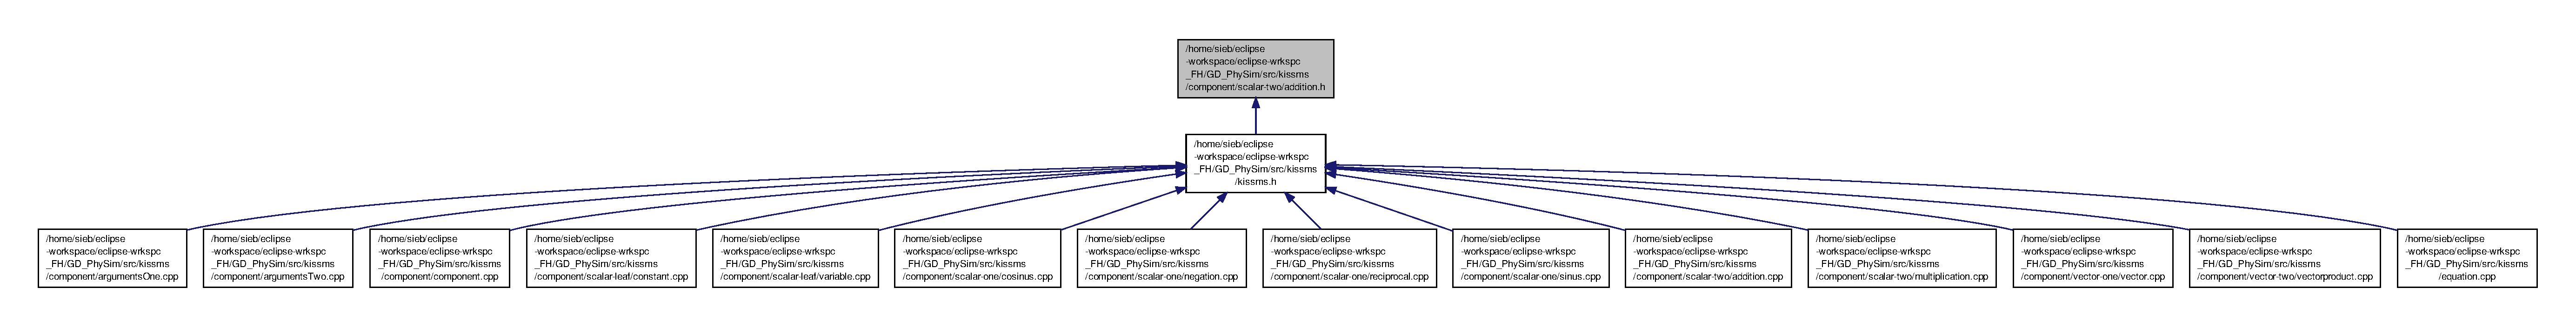
\includegraphics[width=350pt]{addition_8h__dep__incl}
\end{center}
\end{figure}
\subsection*{Classes}
\begin{DoxyCompactItemize}
\item 
class \hyperlink{classkissms_1_1_addition}{kissms\-::\-Addition}
\end{DoxyCompactItemize}
\subsection*{Namespaces}
\begin{DoxyCompactItemize}
\item 
\hyperlink{namespacekissms}{kissms}
\end{DoxyCompactItemize}
\subsection*{Constant Groups}
\begin{DoxyCompactItemize}
\item 
\hyperlink{namespacekissms}{kissms}
\end{DoxyCompactItemize}

\hypertarget{multiplication_8cpp}{\section{/home/sieb/eclipse-\/workspace/eclipse-\/wrkspc\-\_\-\-F\-H/\-G\-D\-\_\-\-Phy\-Sim/src/kissms/component/scalar-\/two/multiplication.cpp File Reference}
\label{multiplication_8cpp}\index{/home/sieb/eclipse-\/workspace/eclipse-\/wrkspc\-\_\-\-F\-H/\-G\-D\-\_\-\-Phy\-Sim/src/kissms/component/scalar-\/two/multiplication.\-cpp@{/home/sieb/eclipse-\/workspace/eclipse-\/wrkspc\-\_\-\-F\-H/\-G\-D\-\_\-\-Phy\-Sim/src/kissms/component/scalar-\/two/multiplication.\-cpp}}
}
{\ttfamily \#include $<$kissms/kissms.\-h$>$}\\*
Include dependency graph for multiplication.\-cpp\-:
\nopagebreak
\begin{figure}[H]
\begin{center}
\leavevmode
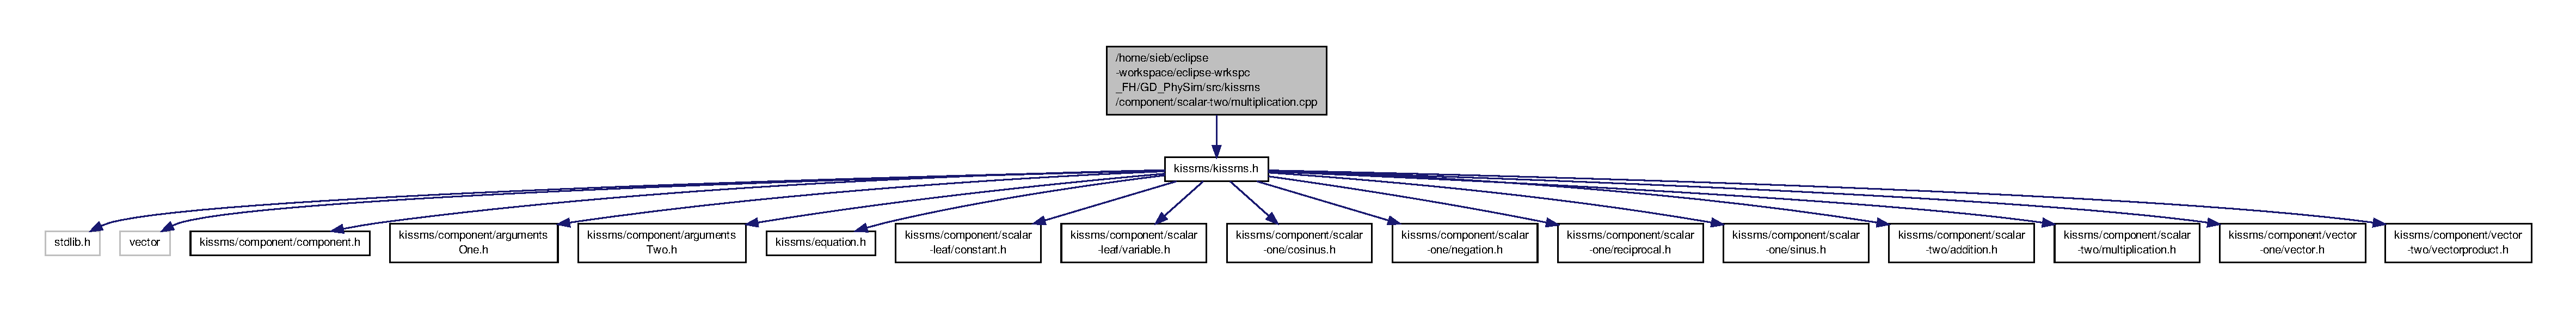
\includegraphics[width=350pt]{multiplication_8cpp__incl}
\end{center}
\end{figure}
\subsection*{Namespaces}
\begin{DoxyCompactItemize}
\item 
\hyperlink{namespacekissms}{kissms}
\end{DoxyCompactItemize}
\subsection*{Constant Groups}
\begin{DoxyCompactItemize}
\item 
\hyperlink{namespacekissms}{kissms}
\end{DoxyCompactItemize}

\hypertarget{multiplication_8h}{\section{/home/sieb/eclipse-\/workspace/eclipse-\/wrkspc\-\_\-\-F\-H/\-G\-D\-\_\-\-Phy\-Sim/src/kissms/component/scalar-\/two/multiplication.h File Reference}
\label{multiplication_8h}\index{/home/sieb/eclipse-\/workspace/eclipse-\/wrkspc\-\_\-\-F\-H/\-G\-D\-\_\-\-Phy\-Sim/src/kissms/component/scalar-\/two/multiplication.\-h@{/home/sieb/eclipse-\/workspace/eclipse-\/wrkspc\-\_\-\-F\-H/\-G\-D\-\_\-\-Phy\-Sim/src/kissms/component/scalar-\/two/multiplication.\-h}}
}
This graph shows which files directly or indirectly include this file\-:
\nopagebreak
\begin{figure}[H]
\begin{center}
\leavevmode
\includegraphics[width=350pt]{multiplication_8h__dep__incl}
\end{center}
\end{figure}
\subsection*{Classes}
\begin{DoxyCompactItemize}
\item 
class \hyperlink{classkissms_1_1_multiplication}{kissms\-::\-Multiplication}
\end{DoxyCompactItemize}
\subsection*{Namespaces}
\begin{DoxyCompactItemize}
\item 
\hyperlink{namespacekissms}{kissms}
\end{DoxyCompactItemize}
\subsection*{Constant Groups}
\begin{DoxyCompactItemize}
\item 
\hyperlink{namespacekissms}{kissms}
\end{DoxyCompactItemize}

\hypertarget{vector_8cpp}{\section{/home/sieb/eclipse-\/workspace/eclipse-\/wrkspc\-\_\-\-F\-H/\-G\-D\-\_\-\-Phy\-Sim/src/kissms/component/vector-\/one/vector.cpp File Reference}
\label{vector_8cpp}\index{/home/sieb/eclipse-\/workspace/eclipse-\/wrkspc\-\_\-\-F\-H/\-G\-D\-\_\-\-Phy\-Sim/src/kissms/component/vector-\/one/vector.\-cpp@{/home/sieb/eclipse-\/workspace/eclipse-\/wrkspc\-\_\-\-F\-H/\-G\-D\-\_\-\-Phy\-Sim/src/kissms/component/vector-\/one/vector.\-cpp}}
}
{\ttfamily \#include $<$kissms/kissms.\-h$>$}\\*
Include dependency graph for vector.\-cpp\-:
\nopagebreak
\begin{figure}[H]
\begin{center}
\leavevmode
\includegraphics[width=350pt]{vector_8cpp__incl}
\end{center}
\end{figure}
\subsection*{Namespaces}
\begin{DoxyCompactItemize}
\item 
\hyperlink{namespacekissms}{kissms}
\end{DoxyCompactItemize}
\subsection*{Constant Groups}
\begin{DoxyCompactItemize}
\item 
\hyperlink{namespacekissms}{kissms}
\end{DoxyCompactItemize}

\hypertarget{vector_8h}{\section{/home/sieb/eclipse-\/workspace/eclipse-\/wrkspc\-\_\-\-F\-H/\-G\-D\-\_\-\-Phy\-Sim/src/kissms/component/vector-\/one/vector.h File Reference}
\label{vector_8h}\index{/home/sieb/eclipse-\/workspace/eclipse-\/wrkspc\-\_\-\-F\-H/\-G\-D\-\_\-\-Phy\-Sim/src/kissms/component/vector-\/one/vector.\-h@{/home/sieb/eclipse-\/workspace/eclipse-\/wrkspc\-\_\-\-F\-H/\-G\-D\-\_\-\-Phy\-Sim/src/kissms/component/vector-\/one/vector.\-h}}
}
This graph shows which files directly or indirectly include this file\-:
\nopagebreak
\begin{figure}[H]
\begin{center}
\leavevmode
\includegraphics[width=350pt]{vector_8h__dep__incl}
\end{center}
\end{figure}
\subsection*{Classes}
\begin{DoxyCompactItemize}
\item 
class \hyperlink{classkissms_1_1_vector}{kissms\-::\-Vector}
\end{DoxyCompactItemize}
\subsection*{Namespaces}
\begin{DoxyCompactItemize}
\item 
\hyperlink{namespacekissms}{kissms}
\end{DoxyCompactItemize}
\subsection*{Constant Groups}
\begin{DoxyCompactItemize}
\item 
\hyperlink{namespacekissms}{kissms}
\end{DoxyCompactItemize}

\hypertarget{vectorproduct_8cpp}{\section{/home/sieb/eclipse-\/workspace/eclipse-\/wrkspc\-\_\-\-F\-H/\-G\-D\-\_\-\-Phy\-Sim/src/kissms/component/vector-\/two/vectorproduct.cpp File Reference}
\label{vectorproduct_8cpp}\index{/home/sieb/eclipse-\/workspace/eclipse-\/wrkspc\-\_\-\-F\-H/\-G\-D\-\_\-\-Phy\-Sim/src/kissms/component/vector-\/two/vectorproduct.\-cpp@{/home/sieb/eclipse-\/workspace/eclipse-\/wrkspc\-\_\-\-F\-H/\-G\-D\-\_\-\-Phy\-Sim/src/kissms/component/vector-\/two/vectorproduct.\-cpp}}
}
{\ttfamily \#include $<$kissms/kissms.\-h$>$}\\*
Include dependency graph for vectorproduct.\-cpp\-:
\nopagebreak
\begin{figure}[H]
\begin{center}
\leavevmode
\includegraphics[width=350pt]{vectorproduct_8cpp__incl}
\end{center}
\end{figure}
\subsection*{Namespaces}
\begin{DoxyCompactItemize}
\item 
\hyperlink{namespacekissms}{kissms}
\end{DoxyCompactItemize}
\subsection*{Constant Groups}
\begin{DoxyCompactItemize}
\item 
\hyperlink{namespacekissms}{kissms}
\end{DoxyCompactItemize}

\hypertarget{vectorproduct_8h}{\section{/home/sieb/eclipse-\/workspace/eclipse-\/wrkspc\-\_\-\-F\-H/\-G\-D\-\_\-\-Phy\-Sim/src/kissms/component/vector-\/two/vectorproduct.h File Reference}
\label{vectorproduct_8h}\index{/home/sieb/eclipse-\/workspace/eclipse-\/wrkspc\-\_\-\-F\-H/\-G\-D\-\_\-\-Phy\-Sim/src/kissms/component/vector-\/two/vectorproduct.\-h@{/home/sieb/eclipse-\/workspace/eclipse-\/wrkspc\-\_\-\-F\-H/\-G\-D\-\_\-\-Phy\-Sim/src/kissms/component/vector-\/two/vectorproduct.\-h}}
}
This graph shows which files directly or indirectly include this file\-:
\nopagebreak
\begin{figure}[H]
\begin{center}
\leavevmode
\includegraphics[width=350pt]{vectorproduct_8h__dep__incl}
\end{center}
\end{figure}
\subsection*{Classes}
\begin{DoxyCompactItemize}
\item 
class \hyperlink{classkissms_1_1_vectorproduct}{kissms\-::\-Vectorproduct}
\end{DoxyCompactItemize}
\subsection*{Namespaces}
\begin{DoxyCompactItemize}
\item 
\hyperlink{namespacekissms}{kissms}
\end{DoxyCompactItemize}
\subsection*{Constant Groups}
\begin{DoxyCompactItemize}
\item 
\hyperlink{namespacekissms}{kissms}
\end{DoxyCompactItemize}

\hypertarget{equation_8cpp}{\section{/home/sieb/eclipse-\/workspace/eclipse-\/wrkspc\-\_\-\-F\-H/\-G\-D\-\_\-\-Phy\-Sim/src/kissms/equation.cpp File Reference}
\label{equation_8cpp}\index{/home/sieb/eclipse-\/workspace/eclipse-\/wrkspc\-\_\-\-F\-H/\-G\-D\-\_\-\-Phy\-Sim/src/kissms/equation.\-cpp@{/home/sieb/eclipse-\/workspace/eclipse-\/wrkspc\-\_\-\-F\-H/\-G\-D\-\_\-\-Phy\-Sim/src/kissms/equation.\-cpp}}
}
{\ttfamily \#include $<$kissms/kissms.\-h$>$}\\*
Include dependency graph for equation.\-cpp\-:
\nopagebreak
\begin{figure}[H]
\begin{center}
\leavevmode
\includegraphics[width=350pt]{equation_8cpp__incl}
\end{center}
\end{figure}
\subsection*{Namespaces}
\begin{DoxyCompactItemize}
\item 
\hyperlink{namespacekissms}{kissms}
\end{DoxyCompactItemize}
\subsection*{Constant Groups}
\begin{DoxyCompactItemize}
\item 
\hyperlink{namespacekissms}{kissms}
\end{DoxyCompactItemize}

\hypertarget{equation_8h}{\section{/home/sieb/eclipse-\/workspace/eclipse-\/wrkspc\-\_\-\-F\-H/\-G\-D\-\_\-\-Phy\-Sim/src/kissms/equation.h File Reference}
\label{equation_8h}\index{/home/sieb/eclipse-\/workspace/eclipse-\/wrkspc\-\_\-\-F\-H/\-G\-D\-\_\-\-Phy\-Sim/src/kissms/equation.\-h@{/home/sieb/eclipse-\/workspace/eclipse-\/wrkspc\-\_\-\-F\-H/\-G\-D\-\_\-\-Phy\-Sim/src/kissms/equation.\-h}}
}
This graph shows which files directly or indirectly include this file\-:
\nopagebreak
\begin{figure}[H]
\begin{center}
\leavevmode
\includegraphics[width=350pt]{equation_8h__dep__incl}
\end{center}
\end{figure}
\subsection*{Classes}
\begin{DoxyCompactItemize}
\item 
class \hyperlink{classkissms_1_1_equation}{kissms\-::\-Equation}
\begin{DoxyCompactList}\small\item\em \hyperlink{classkissms_1_1_component}{Component} representing a whole mathematical equation. \end{DoxyCompactList}\end{DoxyCompactItemize}
\subsection*{Namespaces}
\begin{DoxyCompactItemize}
\item 
\hyperlink{namespacekissms}{kissms}
\end{DoxyCompactItemize}
\subsection*{Constant Groups}
\begin{DoxyCompactItemize}
\item 
\hyperlink{namespacekissms}{kissms}
\end{DoxyCompactItemize}

\hypertarget{kissms_8h}{\section{/home/sieb/eclipse-\/workspace/eclipse-\/wrkspc\-\_\-\-F\-H/\-G\-D\-\_\-\-Phy\-Sim/src/kissms/kissms.h File Reference}
\label{kissms_8h}\index{/home/sieb/eclipse-\/workspace/eclipse-\/wrkspc\-\_\-\-F\-H/\-G\-D\-\_\-\-Phy\-Sim/src/kissms/kissms.\-h@{/home/sieb/eclipse-\/workspace/eclipse-\/wrkspc\-\_\-\-F\-H/\-G\-D\-\_\-\-Phy\-Sim/src/kissms/kissms.\-h}}
}
{\ttfamily \#include $<$stdlib.\-h$>$}\\*
{\ttfamily \#include $<$vector$>$}\\*
{\ttfamily \#include \char`\"{}kissms/component/component.\-h\char`\"{}}\\*
{\ttfamily \#include \char`\"{}kissms/component/arguments\-One.\-h\char`\"{}}\\*
{\ttfamily \#include \char`\"{}kissms/component/arguments\-Two.\-h\char`\"{}}\\*
{\ttfamily \#include \char`\"{}kissms/equation.\-h\char`\"{}}\\*
{\ttfamily \#include \char`\"{}kissms/component/scalar-\/leaf/constant.\-h\char`\"{}}\\*
{\ttfamily \#include \char`\"{}kissms/component/scalar-\/leaf/variable.\-h\char`\"{}}\\*
{\ttfamily \#include \char`\"{}kissms/component/scalar-\/one/cosinus.\-h\char`\"{}}\\*
{\ttfamily \#include \char`\"{}kissms/component/scalar-\/one/negation.\-h\char`\"{}}\\*
{\ttfamily \#include \char`\"{}kissms/component/scalar-\/one/reciprocal.\-h\char`\"{}}\\*
{\ttfamily \#include \char`\"{}kissms/component/scalar-\/one/sinus.\-h\char`\"{}}\\*
{\ttfamily \#include \char`\"{}kissms/component/scalar-\/two/addition.\-h\char`\"{}}\\*
{\ttfamily \#include \char`\"{}kissms/component/scalar-\/two/multiplication.\-h\char`\"{}}\\*
{\ttfamily \#include \char`\"{}kissms/component/vector-\/one/vector.\-h\char`\"{}}\\*
{\ttfamily \#include \char`\"{}kissms/component/vector-\/two/vectorproduct.\-h\char`\"{}}\\*
Include dependency graph for kissms.\-h\-:
\nopagebreak
\begin{figure}[H]
\begin{center}
\leavevmode
\includegraphics[width=350pt]{kissms_8h__incl}
\end{center}
\end{figure}
This graph shows which files directly or indirectly include this file\-:
\nopagebreak
\begin{figure}[H]
\begin{center}
\leavevmode
\includegraphics[width=350pt]{kissms_8h__dep__incl}
\end{center}
\end{figure}
\subsection*{Namespaces}
\begin{DoxyCompactItemize}
\item 
\hyperlink{namespacekissms}{kissms}
\end{DoxyCompactItemize}
\subsection*{Constant Groups}
\begin{DoxyCompactItemize}
\item 
\hyperlink{namespacekissms}{kissms}
\end{DoxyCompactItemize}
\subsection*{Enumerations}
\begin{DoxyCompactItemize}
\item 
enum \hyperlink{namespacekissms_a006cc132ffcae81e38527977e0846e0e}{kissms\-::\-Result\-Code} \{ \hyperlink{namespacekissms_a006cc132ffcae81e38527977e0846e0eaf1e1df84ec126fbfd0baaf448cbd2420}{kissms\-::\-Successful} = 0, 
\hyperlink{namespacekissms_a006cc132ffcae81e38527977e0846e0ea8fc262cf8d89c06412b2293e806b5e29}{kissms\-::\-General\-Failure}, 
\hyperlink{namespacekissms_a006cc132ffcae81e38527977e0846e0eab449d954726399e911403a06e0000a3e}{kissms\-::\-Not\-Yet\-Implemented}
 \}
\end{DoxyCompactItemize}

%--- End generated contents ---

% Index
\newpage
\phantomsection
\addcontentsline{toc}{part}{Index}
\printindex

\end{document}
